\chapter{分形霍尔丹模型理论}
\section{引言}
尽管对拓扑分形绝缘体的兴趣日益增加,但实验实现并不直接,早期尝试\cite{liu2021sierpinski}表明分形性会关闭拓扑性质。直到最近,有一些分形晶格中的拓扑态被实现\cite{kempkes2019design,biesenthal2022fractal,li2023fractal,zhong2024observation,li2023fractality,LI20222040,lai2024spin,ma2023elastic,dorin2024uncovering}。这些进展改变了当前对体-边对应关系的理解:拓扑性质不一定依赖于内部体态。然而,对拓扑分形的物理性质仍处于早期阶段,拓扑相图与分形性之间的相互作用仍然知之甚少。

本章将从一个由两个具有相同数量A和B位点的谢宾斯基三角形组成的分形晶格开始,通过实空间Bott指数\cite{titum2015disorder,wang2020bosonic}和实空间陈数计算相图,我们发现与原始Haldane模型相比,拓扑相图被压缩了约0.5倍。不同代数的拓扑分形晶格的能谱展示了一种自相似的能带层次结构,其形态类似于魔鬼阶梯(康托尔函数)\cite{bak1986devil}。与传统拓扑绝缘体不同,在我们的分形模型中存在一个稳健的迁移率隙,保护拓扑边缘态,而不是直接的带隙。
\section{晶格的产生和维度}
在霍尔丹模型中,AB子晶格的位点势能相反。而三角形外边缘的晶格会造成晶格内位点势能不平衡。对于大尺寸晶格来说,这不会产生太大影响,但如果晶格尺寸较小,此时不平衡的位点势能会造成较强有限尺度效应。因此这里我们采用双Sierpinski三角形作为我们的晶格以平衡位点势能的影响。

在图\ref{fig:FracHaldLatt}中,展示了双Sierpinski三角形晶格的迭代生成过程。每一代Sierpinski三角形G(n)由三个上一代的G(n-1)的副本组成。本文将两个第四代[G(4)]的Sierpinski三角形连接在一起,构成了本文实际讨论的分形晶格。

\begin{figure}
    \centering
    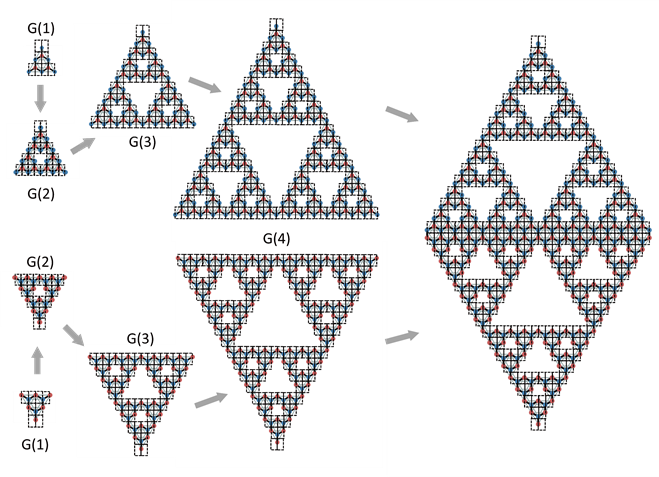
\includegraphics[width=0.75\linewidth]{FracHaldTheo/FracHaldLatt.png}
    \caption{双谢宾斯基三角形晶格的迭代生成}我们的分形晶格由两个第四代(G(4))的Sierpinski三角形组成。每一代Sierpinski三角形G(n)由三个G(n-1)的副本构成。红色和蓝色的点分别表示A和B子晶格。虚线框用于盒计数法以计算晶格的维度。
    \label{fig:FracHaldLatt}
\end{figure}
为了计算分形系统的维度,本文采用了盒计数法。对于每一代迭代,相应的盒数如表\ref{tab:FracHaldLatt}所示。因此,我们的分形系统的维度可以通过下式计算
\begin{equation}
    D = \lim_{n \to \infty} \frac{\ln(N_2)}{\ln(2^{n+1})} = \lim_{n \to \infty} \frac{\ln(4 \times 3^n + 4)}{\ln(2^{n+1})} \approx 1.585
\end{equation}
该值与普通的谢宾斯基三角形一致。
\begin{table}
\centering
\[
\begin{array}{|c|c|c|c|c|c|c|}
\hline
\textbf{迭代次数} & G(1) & G(2) & G(3) & G(4) & \dots & G(n) \\ \hline
\textbf{总盒数}(N_1) & 16 & 40 & 112 & 328 & \dots & 4 \times 3^n + 4 \\ \hline
\textbf{横向盒数}(N_2) & 4 & 8 & 16 & 32 & \dots & 2^{n+1} \\ \hline
\end{array}
\]
\caption{分形晶格每次迭代对应的盒数}在每次迭代中,总盒数$N_1$包括由双 Sierpinski 三角形覆盖的所有盒子。横向盒数 $N_2$包括单个 Sierpinski 三角形边长上的盒子。
\label{tab:FracHaldLatt}
\end{table}


\section{分形霍尔丹模型的哈密顿量}
本节计算采用谢宾斯基三角形晶格上的霍尔丹模型,其哈密顿量可以写作
\begin{equation}
    H = \sum_{\langle ij \rangle} t_1 c_i^\dagger c_j + \sum_{\langle\langle ij \rangle\rangle} t_2 e^{i\phi_{ij}} c_i^\dagger c_j + m \left( \sum_{i \in A} c_i^\dagger c_i - \sum_{i \in B} c_i^\dagger c_i \right) 
\end{equation}
其中 \( c_i^\dagger \) (\( c_{i,j} \)) 是产生(湮灭)算符,$t_1$ 和 $t_2$ 分别是最近邻(NN)和次近邻(NNN)耦合强度,$\phi\_{ij}$ 是从位点 $j$ 跳跃到 NNN 位点 $i$ 时的相位积累,$m$ 表示位点 A 和 B 之间的在位能量差。

\begin{figure}[htbp]
    \centering
    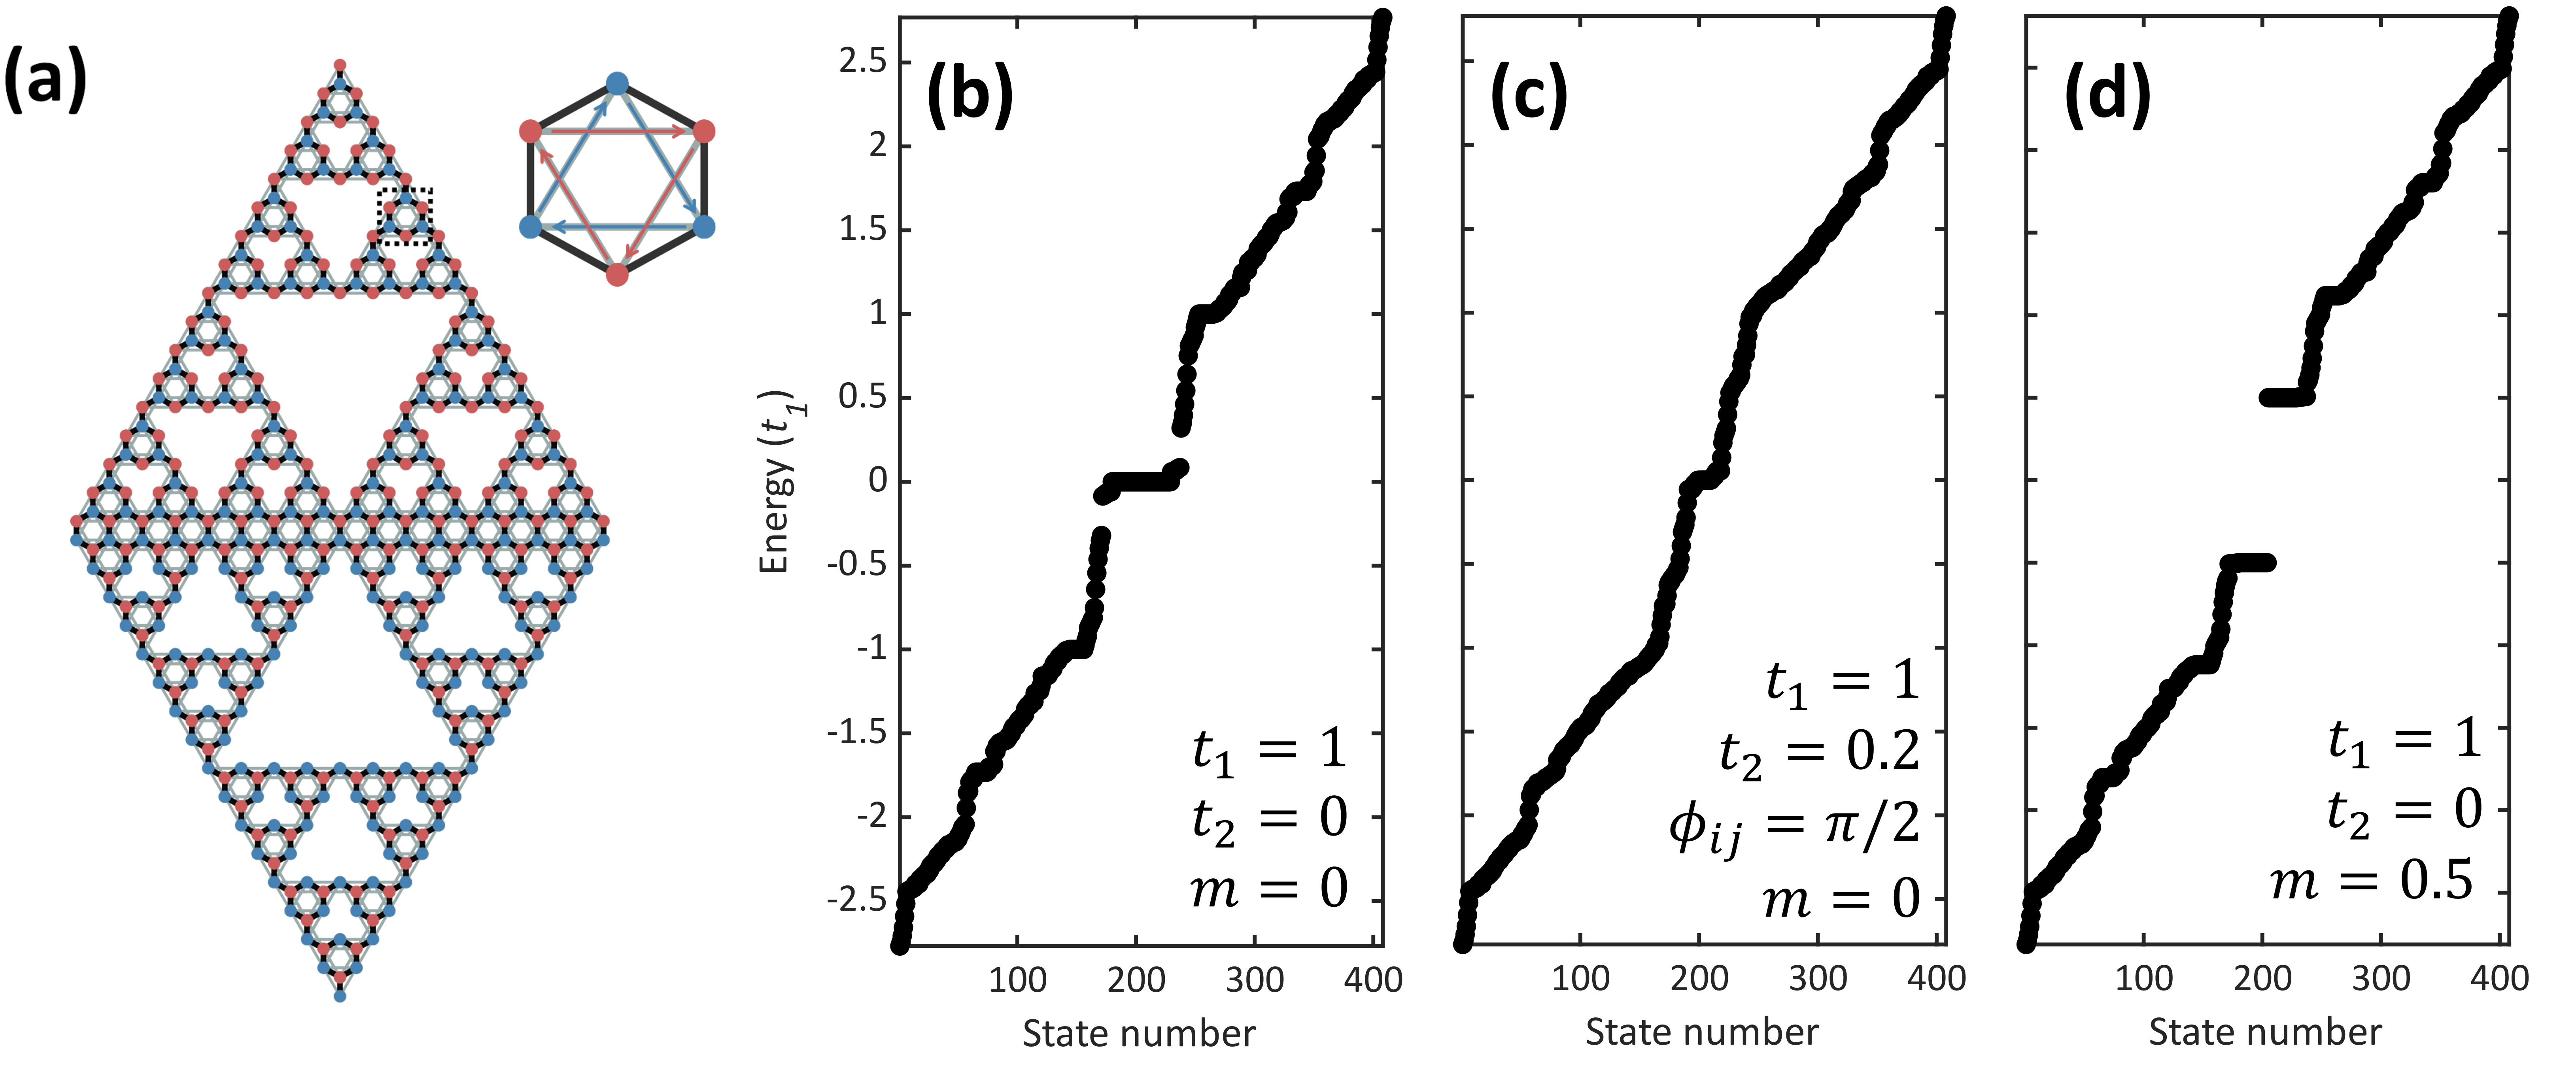
\includegraphics[width=0.75\linewidth]{figure/FracHaldTheo/FractalSpectrum.png}
    \caption{分形晶格与能谱}(a)晶格示意图。插图展示了格点之间的耦合。其中黑线代表NN跃迁$t_1$,灰线代表NNN跃迁$t_2$。箭头代表正耦合相位的方向。蓝色和红色分别代表A和B子晶格。(b-d)分形晶格能谱($t_1=1$)。选取无NNN耦合且无位点势能的情况(b);有NNN耦合的情况($t_2=0.2,\phi=\pi/2$);有位点势能的情况($m=0.5$)。
    \label{fig:FractalSpectrum}
\end{figure}

图\ref{fig:FractalSpectrum}(a)展示了哈密顿量的耦合特征,沿箭头方向跃迁的粒子积累正相位。这些相位的积累在分形晶格中诱发了交错的磁场,打破了晶格的时间反演对称性,带来了非平庸的拓扑相变。如图\ref{fig:FractalSpectrum}(c)所示,相较于仅包含NN耦合的结果[图\ref{fig:FractalSpectrum}(b)],在零能附近出现了无间隙的拓扑边界态。哈密顿量中的位点势能差\( m \)项,打破了晶格的(空间)反演对称性,打开了一个平庸的带隙,如图\ref{fig:FractalSpectrum}(d)所示。需要说明的是,在仅包含NN耦合的例子中,零能处的带与上下的带形成了一个小的带隙,这是由于分形边界对狄拉克点的扰动导致的。

为了进行比较,我们在图\ref{fig:HaldSPec}中展示了蜂窝晶格和分形晶格的能谱图。颜色条表示逆参与率(IPR),其计算公式为 \(\frac{\sum_i |\psi_i|^4}{\left(\sum_i |\psi_i|^2\right)^2}\)(\(i\) 是第 \(i\) 个位点的索引)。较大的 IPR 值表示相应态的局域化行为更强,也即拓扑边缘态的潜在位置。

\begin{figure}[htbp]
    \centering
    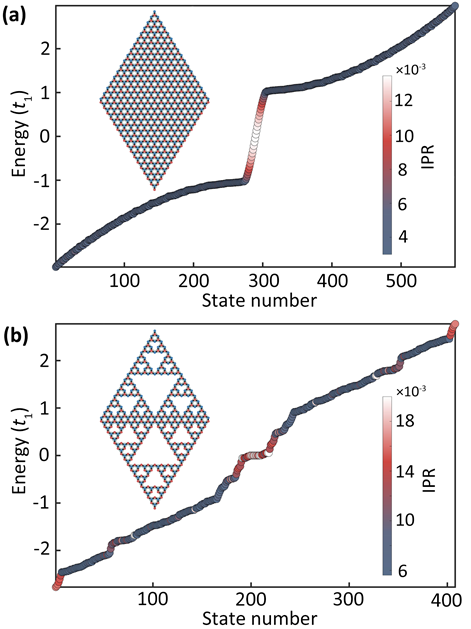
\includegraphics[width=0.45\linewidth]{figure//FracHaldTheo/HaldSPec.png}
    \caption{蜂窝晶格和分形晶格的能谱}本图使用的参数 $\phi$ 和 $m$ 分别为 $\pi/2$ 和 $0$。
    \label{fig:HaldSPec}
\end{figure}

可以看到,由于交错磁场打破了时间反演对称性,二维晶格的霍尔丹模型在零能处产生了一个拓扑带隙,该带隙被高局域度的(IPR标记为洋红和白色)边缘态所填满。同样的结果也可以在分形拓扑绝缘体中观测到,在分形霍尔丹模型的零能处,也出现了许多高局域度的边缘态。与整数维度晶格不同,分形晶格不存在波矢空间,这导致其中心的带隙并不是传统的体带隙,而是类似安德森拓扑绝缘体的迁移率能隙(Mobility gap)。此外,在远离零能处也出现了一些局域的本征态,这些态是由于分形晶格的破缺导致的平庸局域态,而非拓扑边缘态。
\section{分形霍尔丹模型的拓扑不变量}
为了验证我们的分形模型中存在拓扑相变,需要计算拓扑不变量来表征系统。然而,由于分形维度中的空间是碎片化的且缺乏平移对称性,因此无法定义出布洛赫波函数。因此不存在传统的定义在波矢空间的陈数。因此,我们必须将分形晶格投影到二维实空间中,并采用实空间的拓扑不变量:Bott系数\cite{titum2015disorder,wang2020bosonic}和实空间陈数\cite{mitchell2018amorphous}。
\subsection{Bott系数}
Bott 指数是 Loring 和 Hastings 发展出来的一种在应用在凝聚态领域的矩阵指数\cite{hastings2010almost,hastings2011topological}。Bott指数通过投影到环面上的位置矩阵(如下文公式\ref{eq:projectP}所定义)来判断这些矩阵是否可以通过一对可交换矩阵来近似。这编码了关于费米投影P的局域化特性的信息。指数局域化的Wannier函数的存在意味着Bott指数的消失;而Bott指数为零则意味着Wannier函数相对于系统尺寸的方差较小\cite{hastings2011topological}。Bott 指数被用于计算准晶\cite{huang2018quantum}和无序系统\cite{wang2020bosonic}。因此本文采用基于实空间波函数的 Bott 指数来表征缺乏平移对称性的分形系统。Bott系数可以通过以下公式计算\cite{titum2015disorder,wang2020bosonic}:

\begin{equation}
    v_B = \frac{1}{2\pi} \text{Im}\{\text{tr}[\log(UVU^+V^+)]\},
\end{equation}
其中矩阵 \(U\) 和 \(V\) 由以下公式给出:
\begin{equation}
    Pe^{i2\pi X}P = G\begin{pmatrix} 0 & 0 \\ 0 & U \end{pmatrix}G^\dagger,
    \label{eq:projectP}
\end{equation}
\begin{equation}
Pe^{i2\pi Y}P = G\begin{pmatrix} 0 & 0 \\ 0 & V \end{pmatrix}G^\dagger
\end{equation}
其中 \(e^{i2\pi X}\) 和 \(e^{i2\pi Y}\) 是对角酉矩阵。对于大小为 \(N_x\) 和 \(N_y\) 的有限系统,\(\hat{X}\) 和 \(\hat{Y}\) 是位置算子,其对角线元素为 \(i_x/N_x\) 和 \(i_y/N_y\),其中 \(i_{x,y}\) 是晶胞的空间索引。在分块对角矩阵中,第一个块对应于空态,第二个块对应于占据态(由 \(P\) 投影的态)。 \(P\) 是占据态的投影算符,满足
\begin{equation}
P = G\begin{pmatrix} 0 & 0 \\ 0 & I_n \end{pmatrix}G^\dagger
\end{equation}
其中,$n$ 是费米能量下的态数,$I_n$ 是 $n \times n$ 的单位矩阵。$G$ 是 $N \times N$ 的矩阵,其列由哈密顿量的所有本征态组成,并按从 $1$ 到 $N$ 的顺序水平排列,这里 $N$ 是格点数。当系统是拓扑时,Bott 指数为 $1$,否则为0。

我们首先计算二维蜂房晶格霍尔丹模型的结果作为示例。如图\ref{fig:SpecAndBott}(a,b)所示,拓扑态出现在能谱中心的区域,填满了带隙。相应的能量出现了非零的Bott系数和较高的逆参与比(能谱的颜色)。其表明Bott系数可以很好的描述拓扑带隙内的拓扑边缘态。接下来我们计算分形晶格的霍尔丹模型。如图\ref{fig:SpecAndBott}(c,d)所示,在能谱中心的区域,出现了类似于二维蜂房晶格的拓扑边缘态,被Bott系数标记为$+1$。需要注意的是,除了能谱中心的拓扑态外,还出现了一些零散的态被标记为非零的Bott系数。这是由于分形晶格的破缺导致的。这些本征态零散的出现在能谱中,观测其特征模式分布,不具有边缘局域的特性。此外它们也不存在连续的非零带隙,而是在体态范围内突然出现单个孤立的态。因此这里不认为它是拓扑态。
\begin{figure}[htbp]
    \centering
    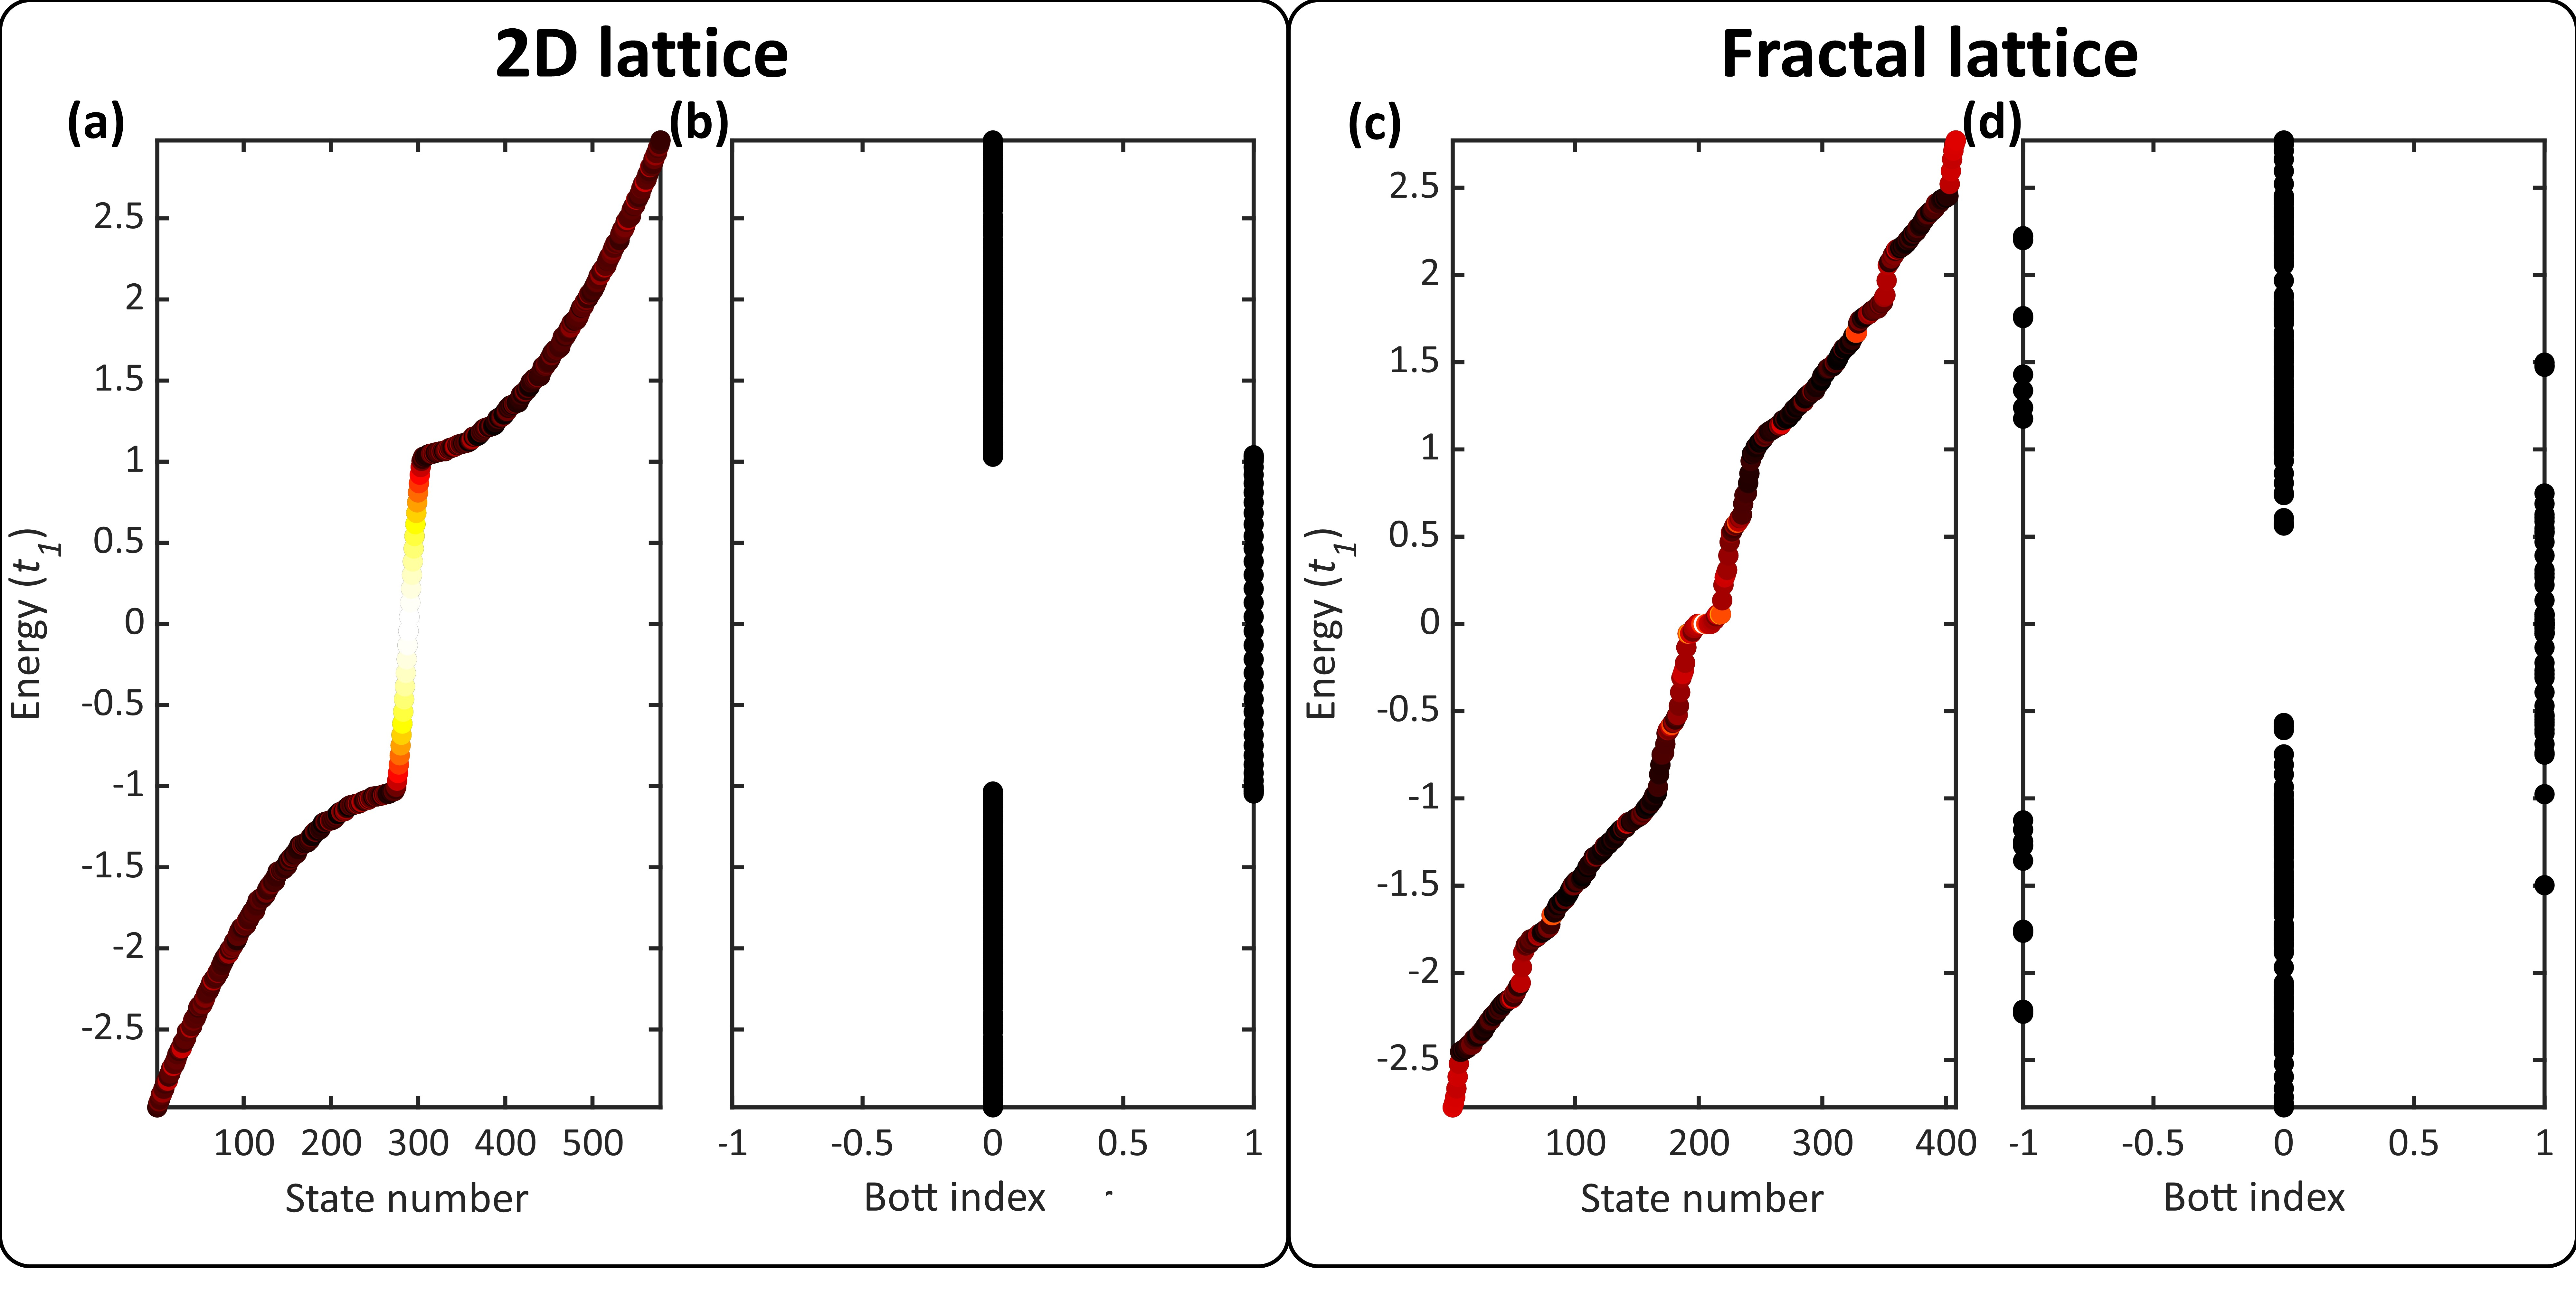
\includegraphics[width=0.75\linewidth]{FracHaldTheo/SpecAndBott.jpg}
    \caption{Bott系数}(a,b)二维晶格的能谱与Bott系数。(c,d)分形晶格的能谱与Bott系数。能谱的颜色为逆参与比。
    \label{fig:SpecAndBott}
\end{figure}
\subsection{实空间陈数}
除Bott系数外,另一种计算在非动量空间中计算陈数的方法是实空间陈数(Real-space Chern numbers)\cite{kitaev2006anyons,mitchell2018amorphous}。其通过投影算符的空间非对易性直接量化系统的拓扑不变量。实空间陈数定义为
\begin{equation}
\nu_{RC} = 12\pi i \sum_{j\in A} \sum_{k\in B} \sum_{l\in C} (P_{jk} P_{kl} P_{lj} - P_{jl} P_{lk} P_{kj})
\end{equation}

其中 \( j, k, l \) 是三个不同相邻区域 \( A, B, C \) 中的位点索引 [如图\ref{fig:RSCN}(a) 所示逆时针排列]。投影算子定义为\( P_{jk} = \langle j|P|k \rangle \),其投影到给定状态。可以发现,该投影算符本质是一个关联矩阵$P_{jk} = \langle j|P|k \rangle$。因此实空间陈数反应了系统的拓扑纠缠熵\cite{kitaev2006topological,levin2006detecting,li2008entanglement,fan2023generalized}。\( A, B, C \)三个区域的尺寸都远大于关联长度。如果任何格点从一个区域重新分配到另一个区域,$\nu_{RC}$ 的值不会改变,因此它是一个拓扑不变量。该定义不依赖于平移不变性,但在平移不变的情况下,它重现了动量空间中熟悉的 TKNN 公式\cite{thouless1982quantized}

\begin{equation}
\nu(P) = \frac{1}{2\pi i} \int \text{tr} \left( \tilde{P} \left( \frac{\partial \tilde{P}}{\partial q_x} \frac{\partial \tilde{P}}{\partial q_y} - \frac{\partial \tilde{P}}{\partial q_y} \frac{\partial \tilde{P}}{\partial q_x} \right) \right) dq_x dq_y
\end{equation}
其中,\(\tilde{P}(q_x, q_y)\) 是 \(P\) 的傅里叶变换,\(\text{tr}(\cdot)\) 表示对能带指标求迹。

我们计算了一个二维蜂房晶格霍尔丹模型,如图\ref{fig:RSCN}(a)所示。图(b)展示了实空间陈数随能量的分布结果,可以看到实空间陈数将能隙内的边缘态识别为1。作为对比,我们计算了Bott系数在图(c)中展示。
\begin{figure}[htbp]
    \centering
    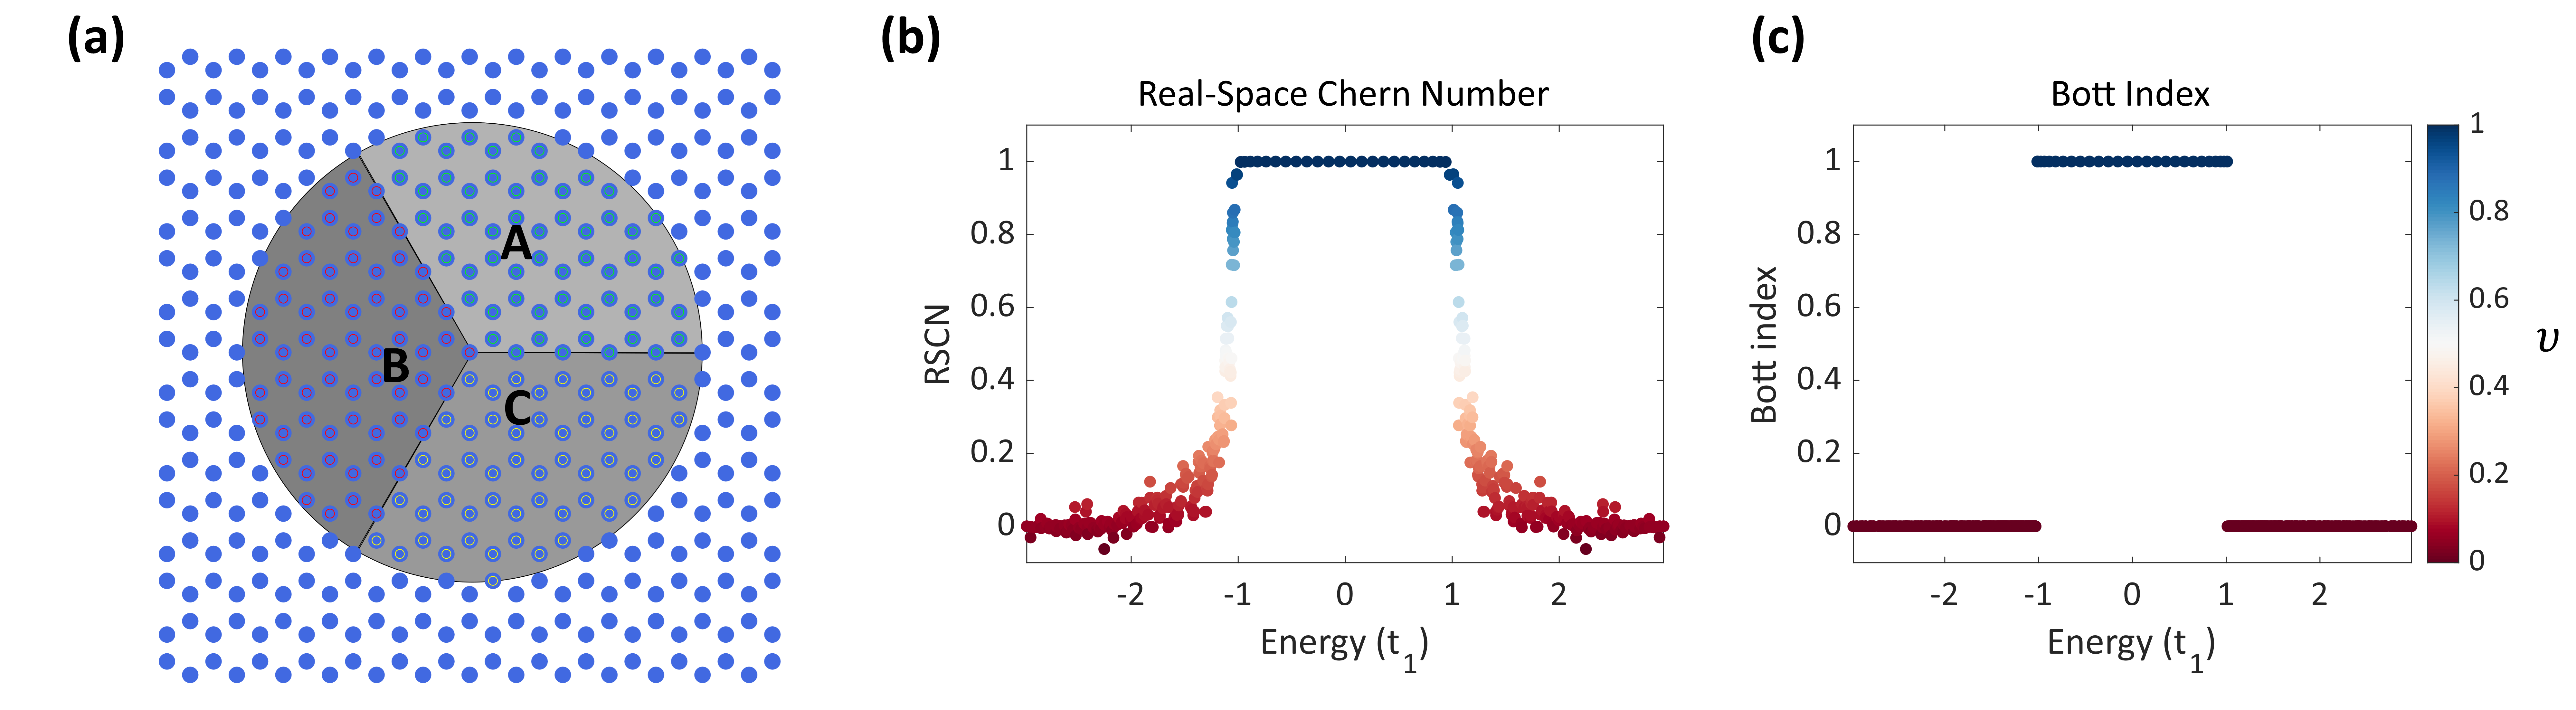
\includegraphics[width=0.75\linewidth]{FracHaldTheo/RSCN.png}
    \caption{实空间陈数}(a)晶格与实空间陈数计算区域。(b)实空间陈数的计算结果。(c)Bott系数的计算结果。
    \label{fig:RSCN}
\end{figure}
由于实空间陈数不需要系统具有平移对称性,其被用于计算准晶\cite{mitchell2018amorphous},无序系统以及分形晶格\cite{yang2020photonic}中的拓扑数。但不同于Bott系数,实空间陈数无法量子化的表明计算的态是0或1,其得到的值是连续分布于区间[0,1]的。因此在后文我们以Bott系数作为主要结果,实空间陈数则作为辅助的验证手段。

\section{能谱Cantor函数和拓扑边缘态}
分形能谱这一概念最早出现于量子霍尔效应中的霍夫斯塔特蝴蝶\cite{hofstadter1976energy}。其分形特性来源于磁场产生的磁原胞与晶格原胞尺寸不匹配。而在分形晶格中,即便缺乏磁原胞,也会出现分形能谱。

在本章的谢宾斯基三角形上的霍尔丹模型中,其边缘态能谱是一个Cantor函数,其也被称为“魔鬼阶梯”。Cantor函数是奇异函数的标准示例。虽然它在所有点上都是连续的,但几乎处处导数为零。康托函数的取值从 0 变化到 1,但在几乎所有点上保持常数。不仅如此,康托函数本身也是一个分形,其维度等于康托集维度的平方\cite{darst1993hausdorff},即 $(\log_2/\log_3)^2 = 0.3981$。
\begin{figure}[htbp]
    \centering
    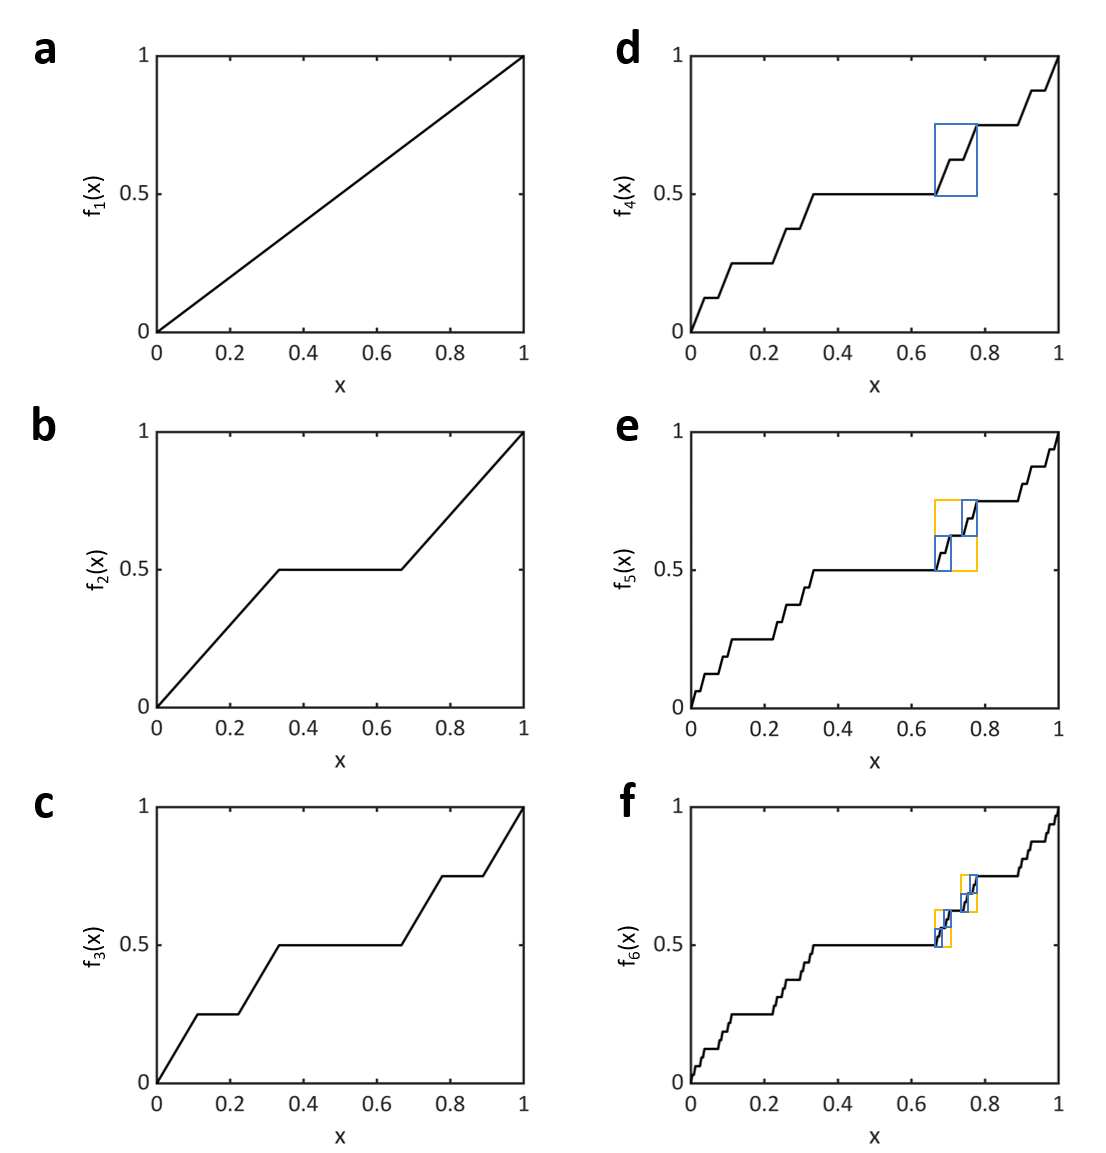
\includegraphics[width=0.5\linewidth]{FracHaldTheo/CantorFunc.png}
    \caption{Cantor函数的迭代生成}(a-f) 迭代函数的步骤 0-5。图\ref{fig:DevStair}中的边缘态的加倍对应于 (d-f) 中的红色和灰色阴影。
    \label{fig:CantorFunc}
\end{figure}
我们可以使用迭代生成康托函数\cite{dovgoshey2006cantor}。首先,定义初始函数 $f_0(x) = x$。然后,每次迭代的下一步函数 $f_{n+1}(x)$ 由前一函数 $f_n(x)$ 定义如下:

\begin{equation}
f_{n+1}(x) =
\begin{cases}
\frac{f_n(3x)}{2}, & x \in \left[0, \frac{1}{3}\right] \\
\frac{1}{2}, & x \in \left[\frac{1}{3}, \frac{2}{3}\right] \\
\frac{1 + f_n(3x - 2)}{2}, & x \in \left[\frac{2}{3}, 1\right]
\end{cases}
\end{equation}

最终,不同步骤的迭代函数如图\ref{fig:CantorFunc}所示。步数 $n$ 取值范围为 0 到 5。图\ref{fig:DevStair}(a-c) 所示的能谱迭代对应于图\ref{fig:CantorFunc},其中边缘态的加倍对应于主文中的红色和灰色阴影。此外,康托函数类型的本征值也出现在树状迭代中\cite{he2003trees}。

我们计算了分形晶格在$\phi=\pi/2,m=0$时的本征值和本征态。G(4-6)的能谱如图\ref{fig:DevStair}(a-c)所示。在能谱中,红色和蓝色点分别表示外部和主导的内部边缘态,如图\ref{fig:DevStair}(g-i)所示。灰色点对应于局域于各种空洞周边的内部边缘态层级,以及由不同迭代代的边缘态组成的混合态层级。分形拓扑绝缘体的一个主要特征在于由分形几何的非平庸切割产生的内部边缘态。这些内部边缘态的出现使得分形拓扑绝缘体完全由“边缘”组成,而没有“体”\cite{yang2020photonic,biesenthal2022fractal}。分形晶格的迭代可以产生越来越多的拓扑边缘态(蓝色、红色和深灰色点),这些态填充了能量区间并生成新的阶梯。例如,在G(5)晶格中,黄色虚线框[图\ref{fig:DevStair}(e)]涵盖了从0.08到0.42的能量范围。它包括从G(4)晶格继承的一个较长的阶梯[图\ref{fig:DevStair}(d)],其能量接近0.28,以及在迭代过程中生成的两个新阶梯,能量分别接近0.12和0.38。连接不同虚线框的近乎平坦的长阶梯包含了许多局域于各种内部空洞周边的内部边缘态。图\ref{fig:DevStair}(d-f)中相同颜色的虚线框具有相似的拓扑边缘态能谱分布。重要的是,我们可以看到,表现出自相似阶梯层级的能谱可以拟合为Cantor函数\cite{Mandelbrot1982,bak1986devil}[见图\ref{fig:DevStair}(a-c)中的灰线]。 

\begin{figure}[htbp]
    \centering
    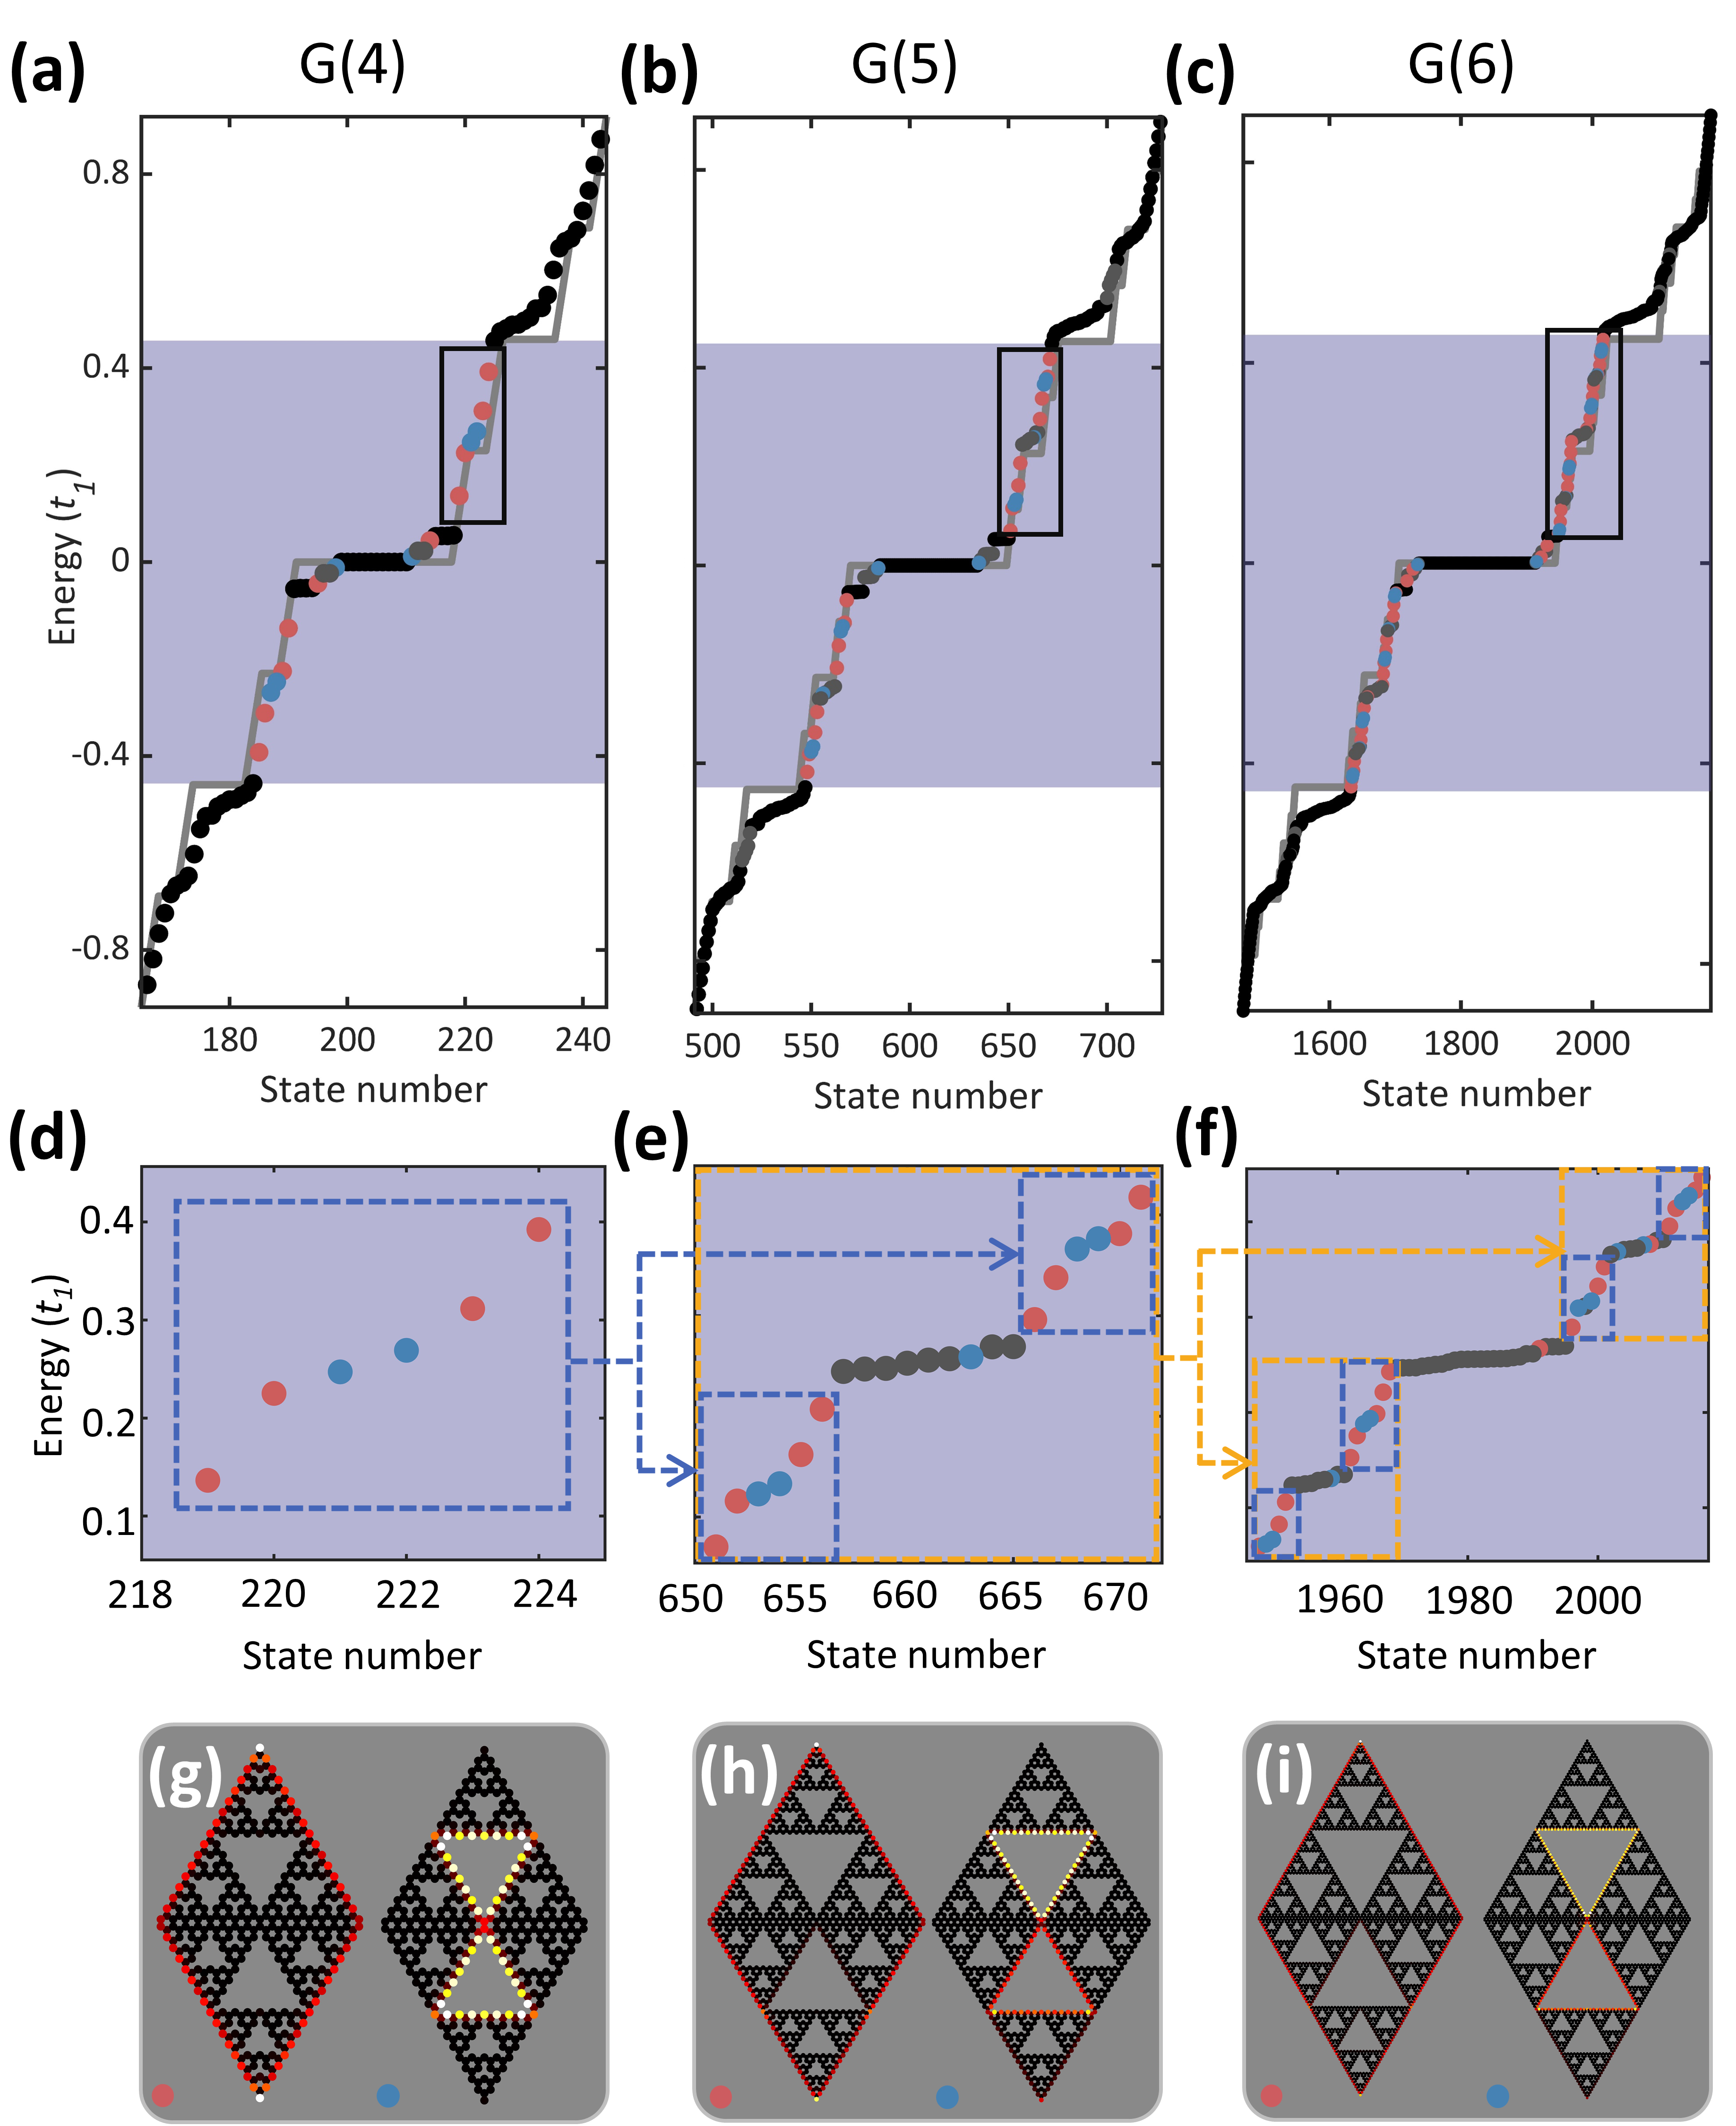
\includegraphics[width=0.5\linewidth]{FracHaldTheo/DevStair.PNG}
    \caption{分形Cantor函数}(a-c) G(4-6)拓扑分形晶格的能量谱。红色和蓝色点分别表示外部和主要内部边缘态,灰色点对应局部于不同空隙边界的层级内部边缘态。蓝色阴影区域表示拓扑带宽,其中可支持拓扑传输。面板 (a-c) 中黑框内的边缘态沿着灰色曲线所示的恶魔阶梯进行迭代。(d-f) 黑框的放大视图,对应于 (a-c) 中的区域。面板 (d-f) 中的蓝色/黄色虚线框在分形晶格的下一代迭代中自身加倍。(g-i) 局部于外部和主要内部边缘的边缘态场模式。外部(内部)边缘态对应的状态编号分别为 224、666、2011(222、654、1950)。
    \label{fig:DevStair}
\end{figure}

能谱分形化的起源是晶格迭代过程中不断产生的内边缘态,这些新的内边缘态会与之前的边缘态简并,形成一系列能谱阶梯。随着阶梯密度增加,不同分布的内边缘态会发生混合,内边缘态和外边缘态也会发生杂化。这带来了一系列特殊的拓扑边缘态。

能谱中的灰色点表示较小的边缘态以及一些混合边缘态。我们以 G(6) 晶格为例,如图\ref{fig:GreyPoint}(a) 所示。我们选择能量接近 0.12 处的灰色阶梯(对应标有箭头‘(b)’的位置),其中的场分布包含一个 G(4) 规模的内部边缘态 [图 \ref{fig:GreyPoint}(b),状态编号 1961],以及一个混合内部边缘态 [图 \ref{fig:GreyPoint}(b),状态编号 1955],该状态局部于 G(4) 和 G(5) 规模区域的边界。类似的结果也出现在能量接近 0.25 处的阶梯上。在这种情况下,G(3) 规模的内部边缘态 [图\ref{fig:GreyPoint}(c),状态编号 1983 和 1992] 与另一个包含 G(3)、G(4) 和 G(5) 三种尺度的内部边缘态 [图\ref{fig:GreyPoint}(c),状态编号 1987] 同时共存。
\begin{figure}[htbp]
    \centering
    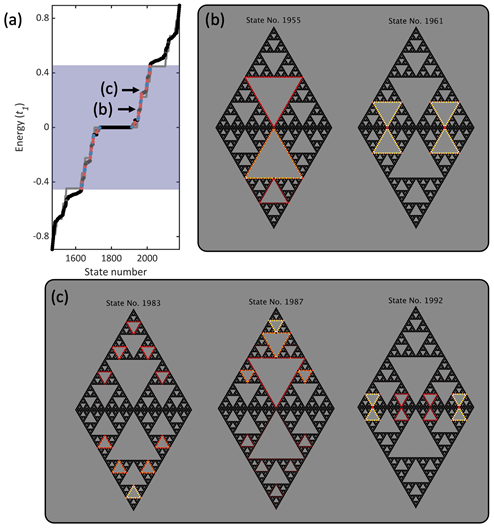
\includegraphics[width=0.5\linewidth]{FracHaldTheo/GreyPoint.png}
    \caption{混合边缘态}(a)G(6)晶格的能谱。(b,c)能量为0.12(b)和0.25(c)的场分布。对应于(a)中的黑色箭头。
    \label{fig:GreyPoint}
\end{figure}

混合边缘态是单个本征态,但分布于不同的迭代的内边缘上。除了混合边缘态外,不同迭代的内边缘还会由于简并而形成簇态(cluster states)。那么用简并能量激励系统时,其动力学特性如何。在实验中实现簇态具有挑战性。簇态的出现需要较长的演化时间,我们将在下文中通过数值结果加以证明。

由于这些简并态的空间重叠度较低,在早期阶段只能优先激发一个边缘态。如图 \ref{fig:TimeEvoCluster}(a) 所示,在经过 200 秒的演化后,态仍然局限于最大内边缘。激发位置由蓝色点标记。

\begin{figure}[htbp]
    \centering
    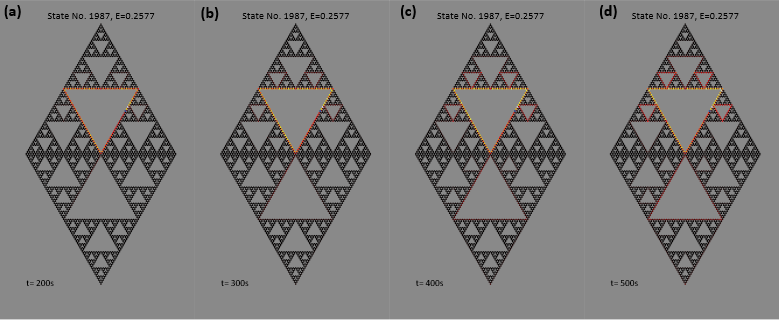
\includegraphics[width=0.75\linewidth]{FracHaldTheo/TimeEvoCluster.png}
    \caption{混合边缘态的时间演化}(a-d) 在$t=200,300,400,500$秒时的场分布。经过 200 秒的演化(图 a),场分布仍然局限于最大内边缘。随着时间的推移,场分布逐渐扩展到其他简并本征态。
    \label{fig:TimeEvoCluster}
\end{figure}

而当演化时间足够长,如图\ref{fig:TimeEvoCluster}(b-d) 所示,这种簇态是可激发的。本节选择了本征能量为$E=0.2577$的阶梯进行分析。

除了在图\ref{fig:GreyPoint}中展示的内边缘混合态外,还可能发生内边缘态和外边缘态的杂化。在 G(4) 晶格中,内边缘态和外边缘态的本征能量差较大[图\ref{fig:HybridState}(a)],因此不会发生杂化。而当晶格的代数增加,例如 G(6),会出现越来越多的本征态[图\ref{fig:HybridState}(b)],并填充蓝色拓扑区域内的拓扑能隙。因此,内边缘态和外边缘态可能具有足够接近的本征能量,从而这些本征态可以在近平坦的阶梯上发生杂化。

在图\ref{fig:HybridState}(c) 中,我们展示了第 1995 号态的杂化本征态。该杂化边缘态的场分布局限于外边缘以及 G(3) 规模的内边缘。
\begin{figure}[htbp]
    \centering
    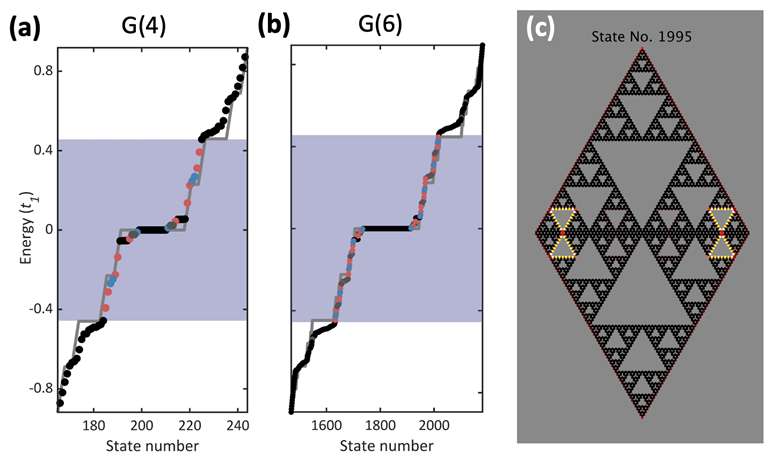
\includegraphics[width=0.75\linewidth]{FracHaldTheo/HybridState.png}
    \caption{内外边缘的杂化态}(a, b) G(4) 和 G(6) 晶格的能谱。红色和蓝色点分别表示外部边缘态和主要的内部边缘态。灰色点对应于局限于不同空隙边界的层级化内部边缘态。(c) 杂化边缘态的场分布,该态局限于外部边缘和 G(3) 规模的内部边缘。
    \label{fig:HybridState}
\end{figure}

在能谱 [图\ref{fig:SuspEdge}(a)] 中,存在一些可疑的拓扑边缘态。例如,在 (a) 图中由红色箭头 (e) 指出的本征态 235 [图\ref{fig:SuspEdge}(e)] 的场分布看起来像是拓扑边缘态。然而,动力学模拟表明,态 235 无法支持单向传输,而不会渗透到晶格内部。需要注意的是,在模拟中,我们在边缘放置了一个点源,以态 212 和态 235 的能量发射波。

在 (b-d) 图中,我们展示了一些典型的平庸态(trivial states)的场分布,这些态的能量接近 0,处于稳健的迁移能隙(蓝色阴影区域)之内。这些态是平庸态,并局限于内部空隙的边界。
\begin{figure}[htbp]
    \centering
    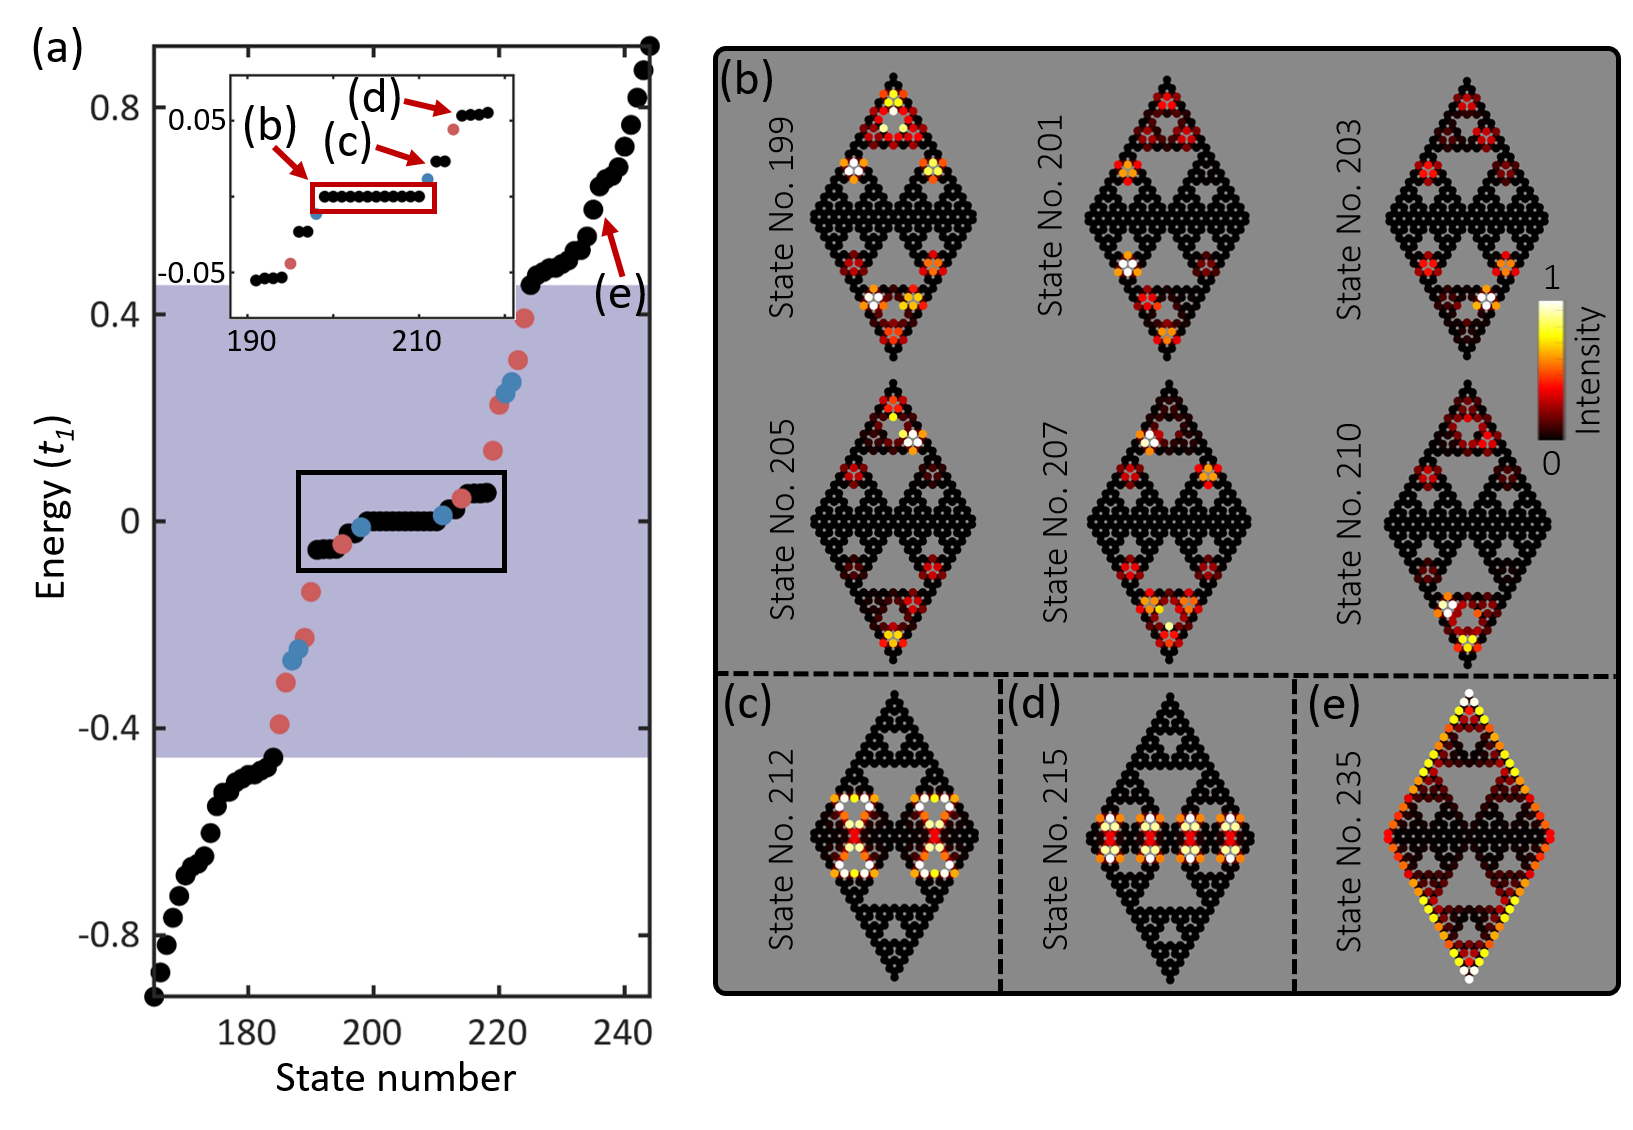
\includegraphics[width=0.75\linewidth]{FracHaldTheo/SuspEdge.png}
    \caption{可疑的边缘态}
    \label{fig:SuspEdge}(a) G(4)晶格的能谱。(b-d) 能量接近 0 的平庸态的典型场分布。(e) 一个可疑的拓扑态。该态可以渗透到晶格内部,并且不受拓扑保护。
\end{figure}

{\color{red}众所周知,在传统拓扑绝缘体中,拓扑边界态仅存在于带隙内。然而,在我们的分形模型中,即使在能量接近 0 的平庸态存在的情况下,拓扑传播仍能保持稳定(见补充材料,电影 3-5)。其原因在于,由于缺乏明确定义的体态,边界态与局域于内部空隙周围的态之间的耦合可以忽略不计。因此,存在一个从 $-0.46$ 到 $0.46$ 的稳健迁移能隙(对应于图 2(a-c) 中蓝色阴影区域),其 Bott 指数为 1,该能隙保护拓扑边界态,而非直接的带隙,使得我们的分形模型在根本上不同于传统拓扑能带绝缘体。需要注意的是,在补充材料的电影 6 中,我们还展示了拓扑传输能够保持的条件:只要边界围绕的区域大于 $G(2)$,拓扑传输仍然存在。由于有限尺寸效应,围绕较小区域的边界无法支持单向传输。}

\section{压缩的拓扑相图}
在原始的 Haldane 模型中,两种对称性破缺之间的竞争可以引发拓扑相变,如图 \ref{fig:SqueezedPhase}(b, c) 中的灰色线所示。直观上,人们可能会想知道我们的分形系统中是否存在拓扑相变,以及相变的位置在哪里。

Bott 指数的计算结果作为参数$\phi$和$m$的函数,展示在图\ref{fig:SqueezedPhase}(b, c) 中。为了进行直接比较,我们分别计算了蜂窝晶格 [图\ref{fig:SqueezedPhase}(b)] 和我们的分形晶格 [图\ref{fig:SqueezedPhase}(c)] 的相图。Haldane 模型中由$|m|=|3\sqrt{3}t_2sin\phi|$控制的著名拓扑相变在两幅图中均以灰色线标出。这些线连接了两个具有不同 Chern 数$\nu$的区域,Chern 数$\nu$从 0 变化为 +1 或 -1。

\begin{figure}[htbp]
    \centering
    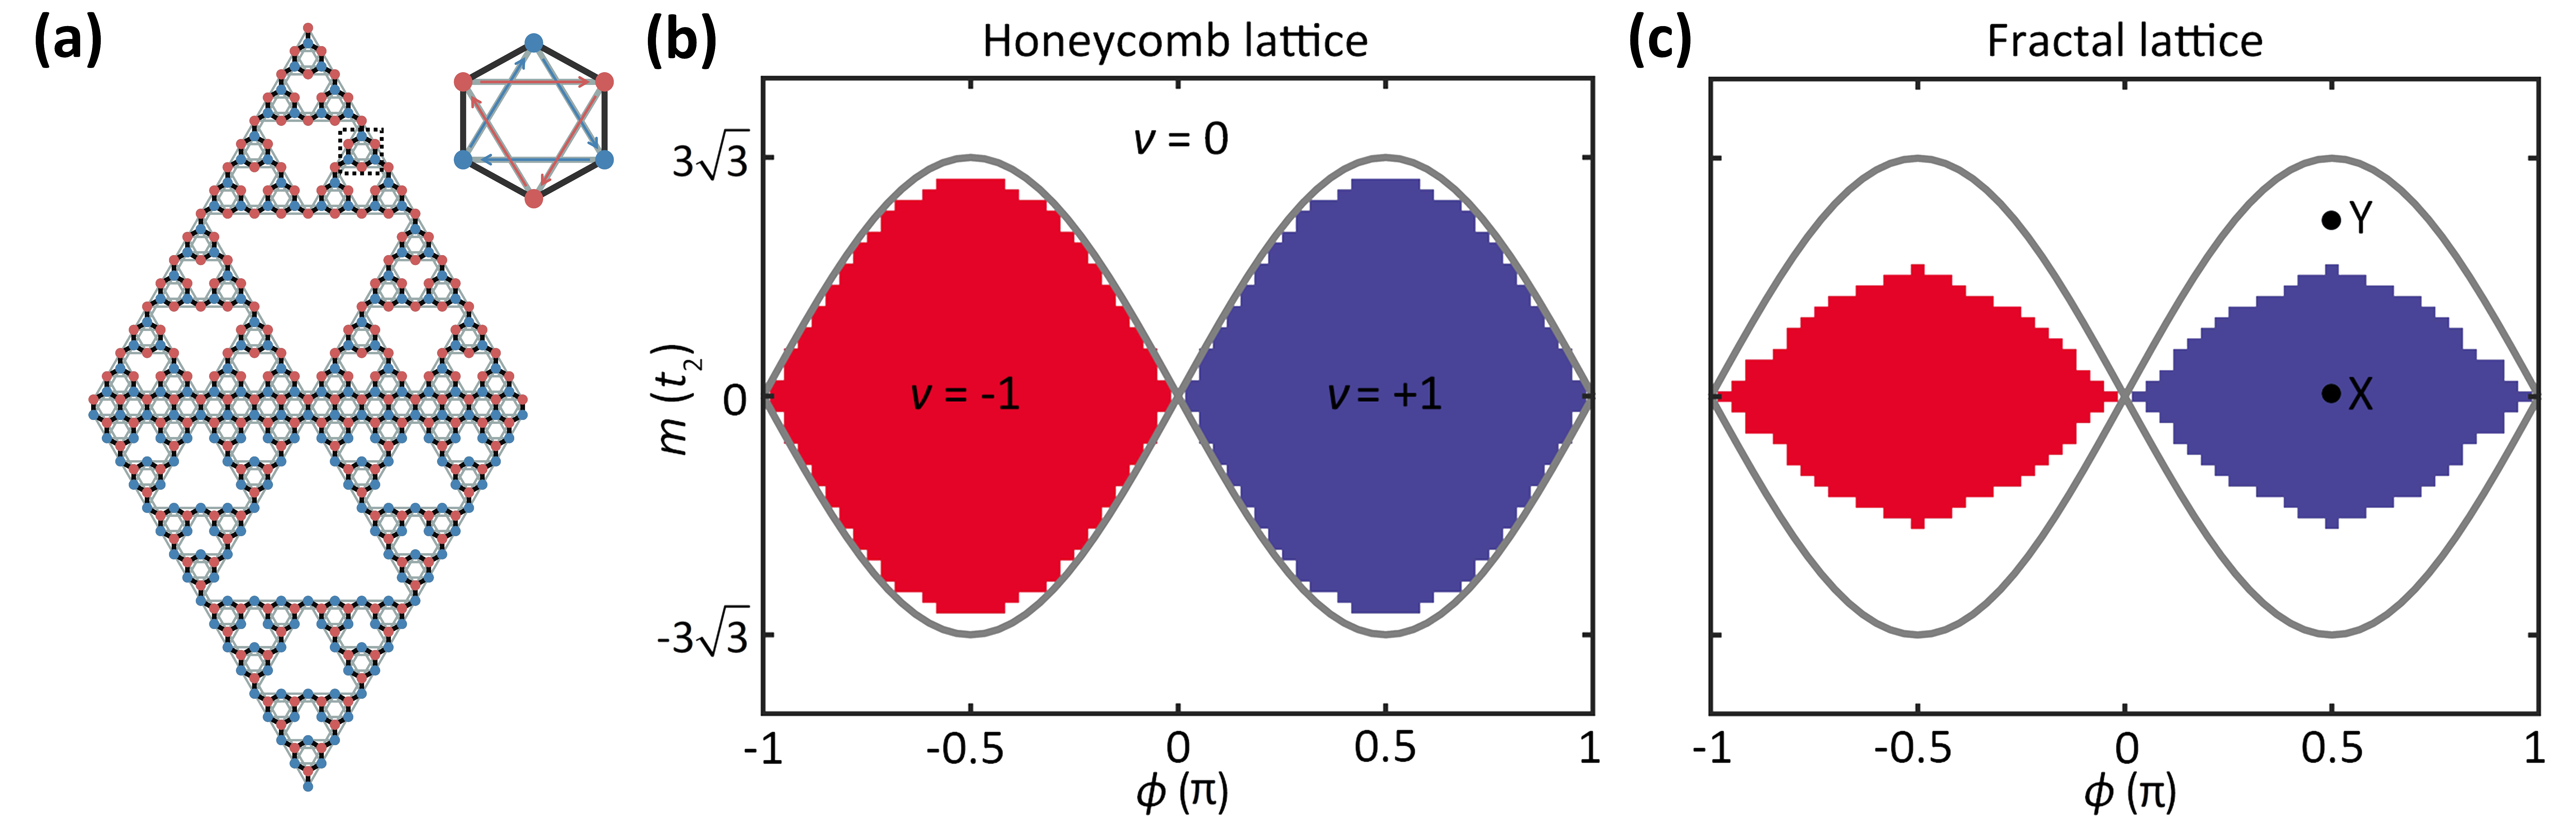
\includegraphics[width=0.75\linewidth]{FracHaldTheo/SqueezedPhase.PNG}
    \caption{压缩的拓扑相图}\textbf{(a)} 示意图展示了由两个 Sierpinski三角形组成的分形 Haldane 模型。红色和蓝色点分别表示 A 和 B 亚晶格,且它们包含相同数量的晶格点。最近邻和次近邻耦合分别用黑色和灰色线表示。沿红色或蓝色箭头的次近邻跳跃可积累一个相位 $\phi$。插图为六边形单元的放大图。\textbf{(b)} 菱形蜂窝晶格的拓扑相图。在原始 Haldane 模型中,拓扑相变遵循$|m| = |3\sqrt{3} t_2 \sin \phi|$该相变关系由灰色线标记。Bott 指数 0、+1 和 -1 分别用白色、蓝色和红色表示。\textbf{(c)} 分形晶格的相图沿垂直轴 $m$ 被显著压缩约 0.5 倍。理论计算的耦合参数为:$t_1 = 1$,$t_2 = 0.2$。
    \label{fig:SqueezedPhase}
\end{figure}

对于蜂窝晶格 [图\ref{fig:SqueezedPhase}(b)],Bott 指数计算得到的相图与由 Chern 数计算的结果一致。Bott 指数 0、+1 和 -1 分别用白色、蓝色和红色表示。Bott 指数$\pm1$和 0 之间的相变与理论预测(灰色线)相吻合。而对于分形晶格,相图 [图\ref{fig:SqueezedPhase}(c)] 沿垂直轴$m$被大约 0.5 倍压缩,这是由于晶格格点数量减少,使得需要较小的反演对称性破缺来平衡时间反演对称性破缺。

拓扑相图的压缩现象可以通过拓扑边缘态的场分布来证明。接下来笔者将举一个存在交错势能差但拓扑的例子($\phi = \pi/2, m = 1.6t_2$)以及一个二维蜂房晶格拓扑,但分形晶格平庸的例子($\phi = \pi/2, m = 3.6t_2$)。

在 $\phi = \pi/2$ 和 $m = 1.6t_2$ 的条件下,蜂窝晶格和分形晶格中均存在对应于非零 Bott 指数的拓扑边缘态。场分布如图\ref{fig:TransitionEdge}(a, c, e) 所示。当 $\phi = \pi/2$ 且 $m = 3.6t_2$ 时,蜂窝晶格处于拓扑相,而分形晶格处于平庸相,此时仅在蜂窝晶格中可以找到拓扑边缘态,而在分形晶格中则无法找到此类态。在图 (d, f) 中,绘制了一个可疑的拓扑边缘态(编号 175 和 176)的场分布。我们通过模拟确认,态 175 和 176 无法支持拓扑输运。

\begin{figure}[htbp]
    \centering
    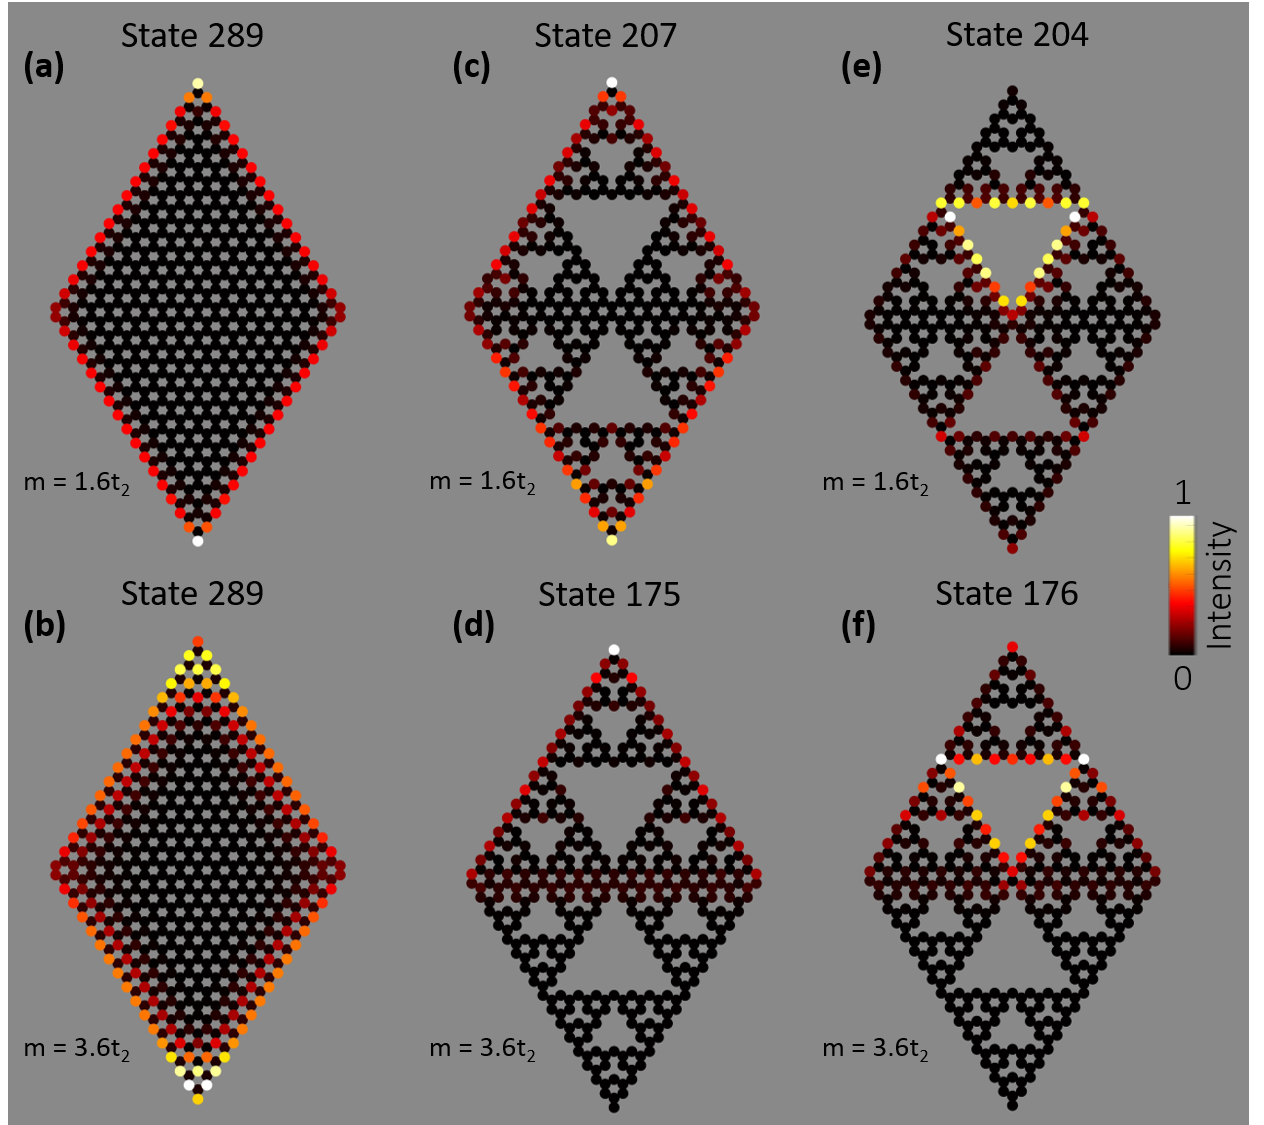
\includegraphics[width=0.5\linewidth]{FracHaldTheo/TransitionEdge.png}
    \caption{本征态的拓扑相变}(a, c, e) 边缘态的场分布,对应于 $\phi = \pi/2$ 和 $m = 1.6t_2$ 条件下蜂窝晶格和分形晶格中 Bott 指数为 1 的状态。(b, d, f) 边缘态及可疑边缘态的场分布,分别对应于 $\phi = \pi/2$ 和 $m = 3.6t_2$ 条件下蜂窝晶格中 Bott 指数为 1 的状态和分形晶格中 Bott 指数为 0 的状态。
    \label{fig:TransitionEdge}
\end{figure}

小尺寸晶格的结果可能会具有较强的有限尺度效应。例如图\ref{fig:SqueezedPhase}(b)中的二维蜂房晶格,其包含了289个格点,于G(4)晶格具有相同尺寸的外边缘。其Bott系数计算出的拓扑相图区域略小于k空间计算出的拓扑相图区域。

为了排除有限尺度效应的影响,并检验分形不同迭代次数下拓扑相图的一致性,我们计算了 G(3)、G(4) 和 G(5) 三个代数的相图。正如图\ref{fig:G(4-6)Phase}(d-f) 所示,尽管在相图边缘存在一些小的波动,这些相图的总体范围仍表现出良好的一致性。

\begin{figure}[htbp]
    \centering
    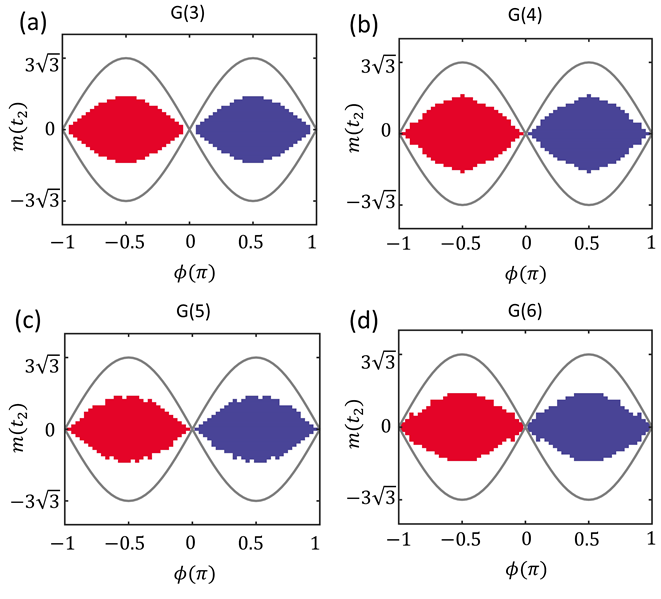
\includegraphics[width=0.5\linewidth]{FracHaldTheo/G(4-6)Phase.png}
    \caption{不同迭代的拓扑相图}(a-d) G(3)、G(4) 和 G(5) 晶格的拓扑相图。Bott 指数 0、+1 和 -1 分别用白色、蓝色和红色表示。理论计算的耦合参数为:$t_1 = 1$,$t_2 = 0.2$。
    \label{fig:G(4-6)Phase}
\end{figure}

上述相图均选取Bott系数作为拓扑不变量,这是由于分形晶格缺乏平移对称性,没有良好定义的k空间,因此需要利用Bott系数来替代k空间陈数作为分形晶格的拓扑不变量。而除了Bott系数外,非平移对称系统的拓扑性质还可以通过实空间陈数来表征。为了进一步验证Bott系数和压缩相图的有效性,本节计算了特定参数下的实空间陈数的结果。

实空间陈数捕捉了波函数的关联性质。因此类似于拓扑纠缠熵的计算,实空间陈数也需要选取三个不同的区域来计算相应的投影算符。本文选取的投影算符区域如图\ref{fig:RSCNPhase}(a)的灰色区域所示。 

\begin{figure}[htbp]
    \centering
    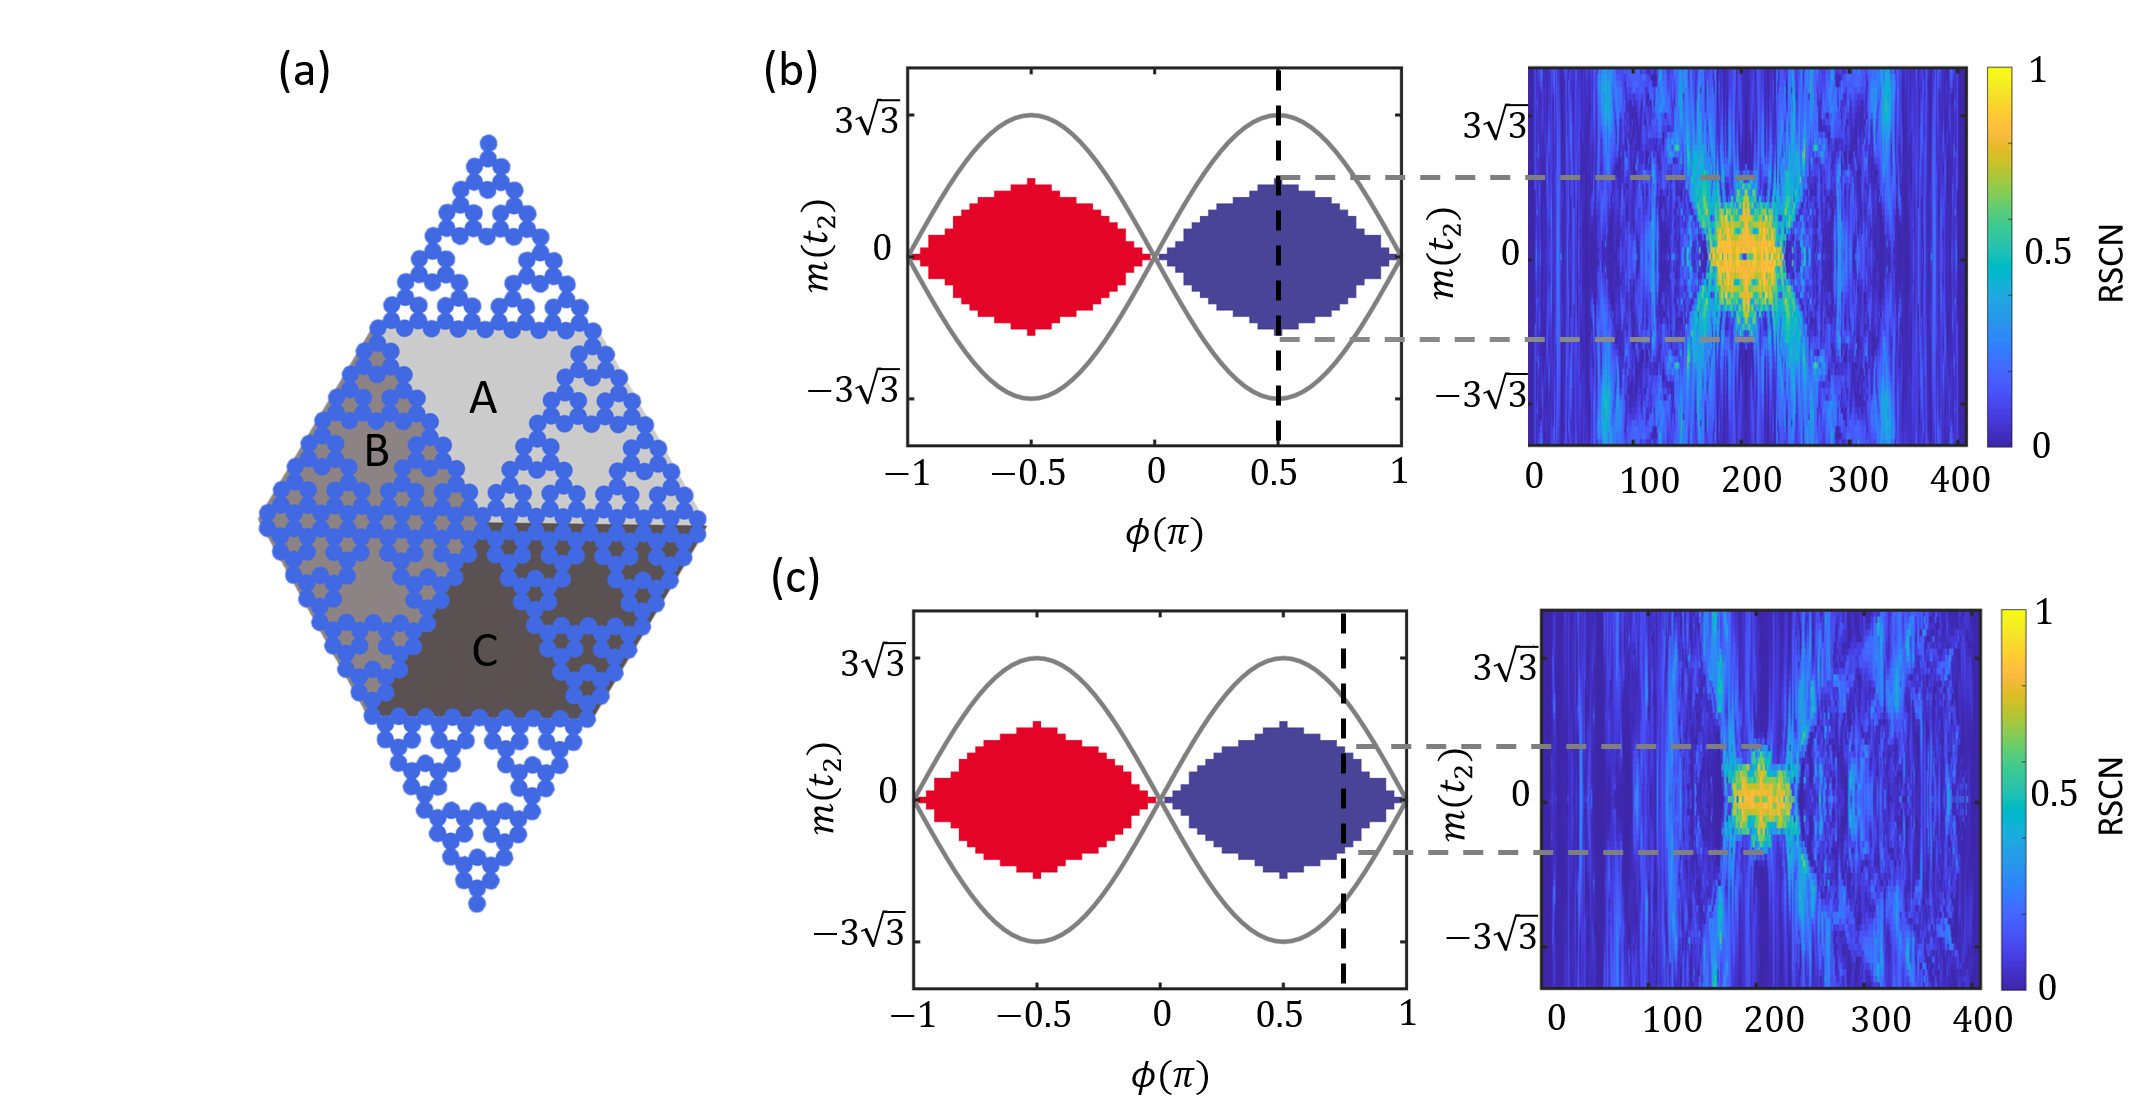
\includegraphics[width=0.75\linewidth]{FracHaldTheo/RSCNPhase.png}
    \caption{压缩拓扑相图的实空间陈数验证}(a) 实空间陈数计算的示意图。(b, c) 由 Bott 指数计算得到的拓扑相图显示在左侧面板。Bott 指数 0、+1 和 -1 分别用白色、蓝色和红色表示。在右侧两个面板中,我们计算了沿两条黑色虚线(分别对应于$\phi=\pi/2$和$\phi=3\pi/4$)的实空间陈数。
    \label{fig:RSCNPhase}
\end{figure}

在图\ref{fig:RSCNPhase}(b, c) 中,我们计算了对应于$\phi=\pi/2$和$\phi=3\pi/4$的两条黑色虚线上的实空间陈数。在右侧的两个面板中,我们展示了基于实空间陈数计算的结果,实空间陈数以本征态编号和交错势能差为函数表示。

黄色区域对应于实空间 Chern 数为 1。可以看到,沿垂直轴(交错势能差)的拓扑相变与 Bott 指数方法计算得到的结果具有良好的一致性,Bott 指数计算结果由水平灰色虚线标示。

拓扑相变的另一个证据是拓扑带隙(迁移率隙)的关闭。在本节中,笔者展示了蜂窝晶格和分形晶格的拓扑带隙图。如图\ref{fig:BandGap}(a,b)所示,颜色条表示带隙的大小。带隙大小通过求和所有具有 Bott 指数 1 的态n与其相邻态n+1之间的小带隙来确定,如图\ref{fig:BandGap}(c,d)所示。

\begin{figure}[htbp]
    \centering
    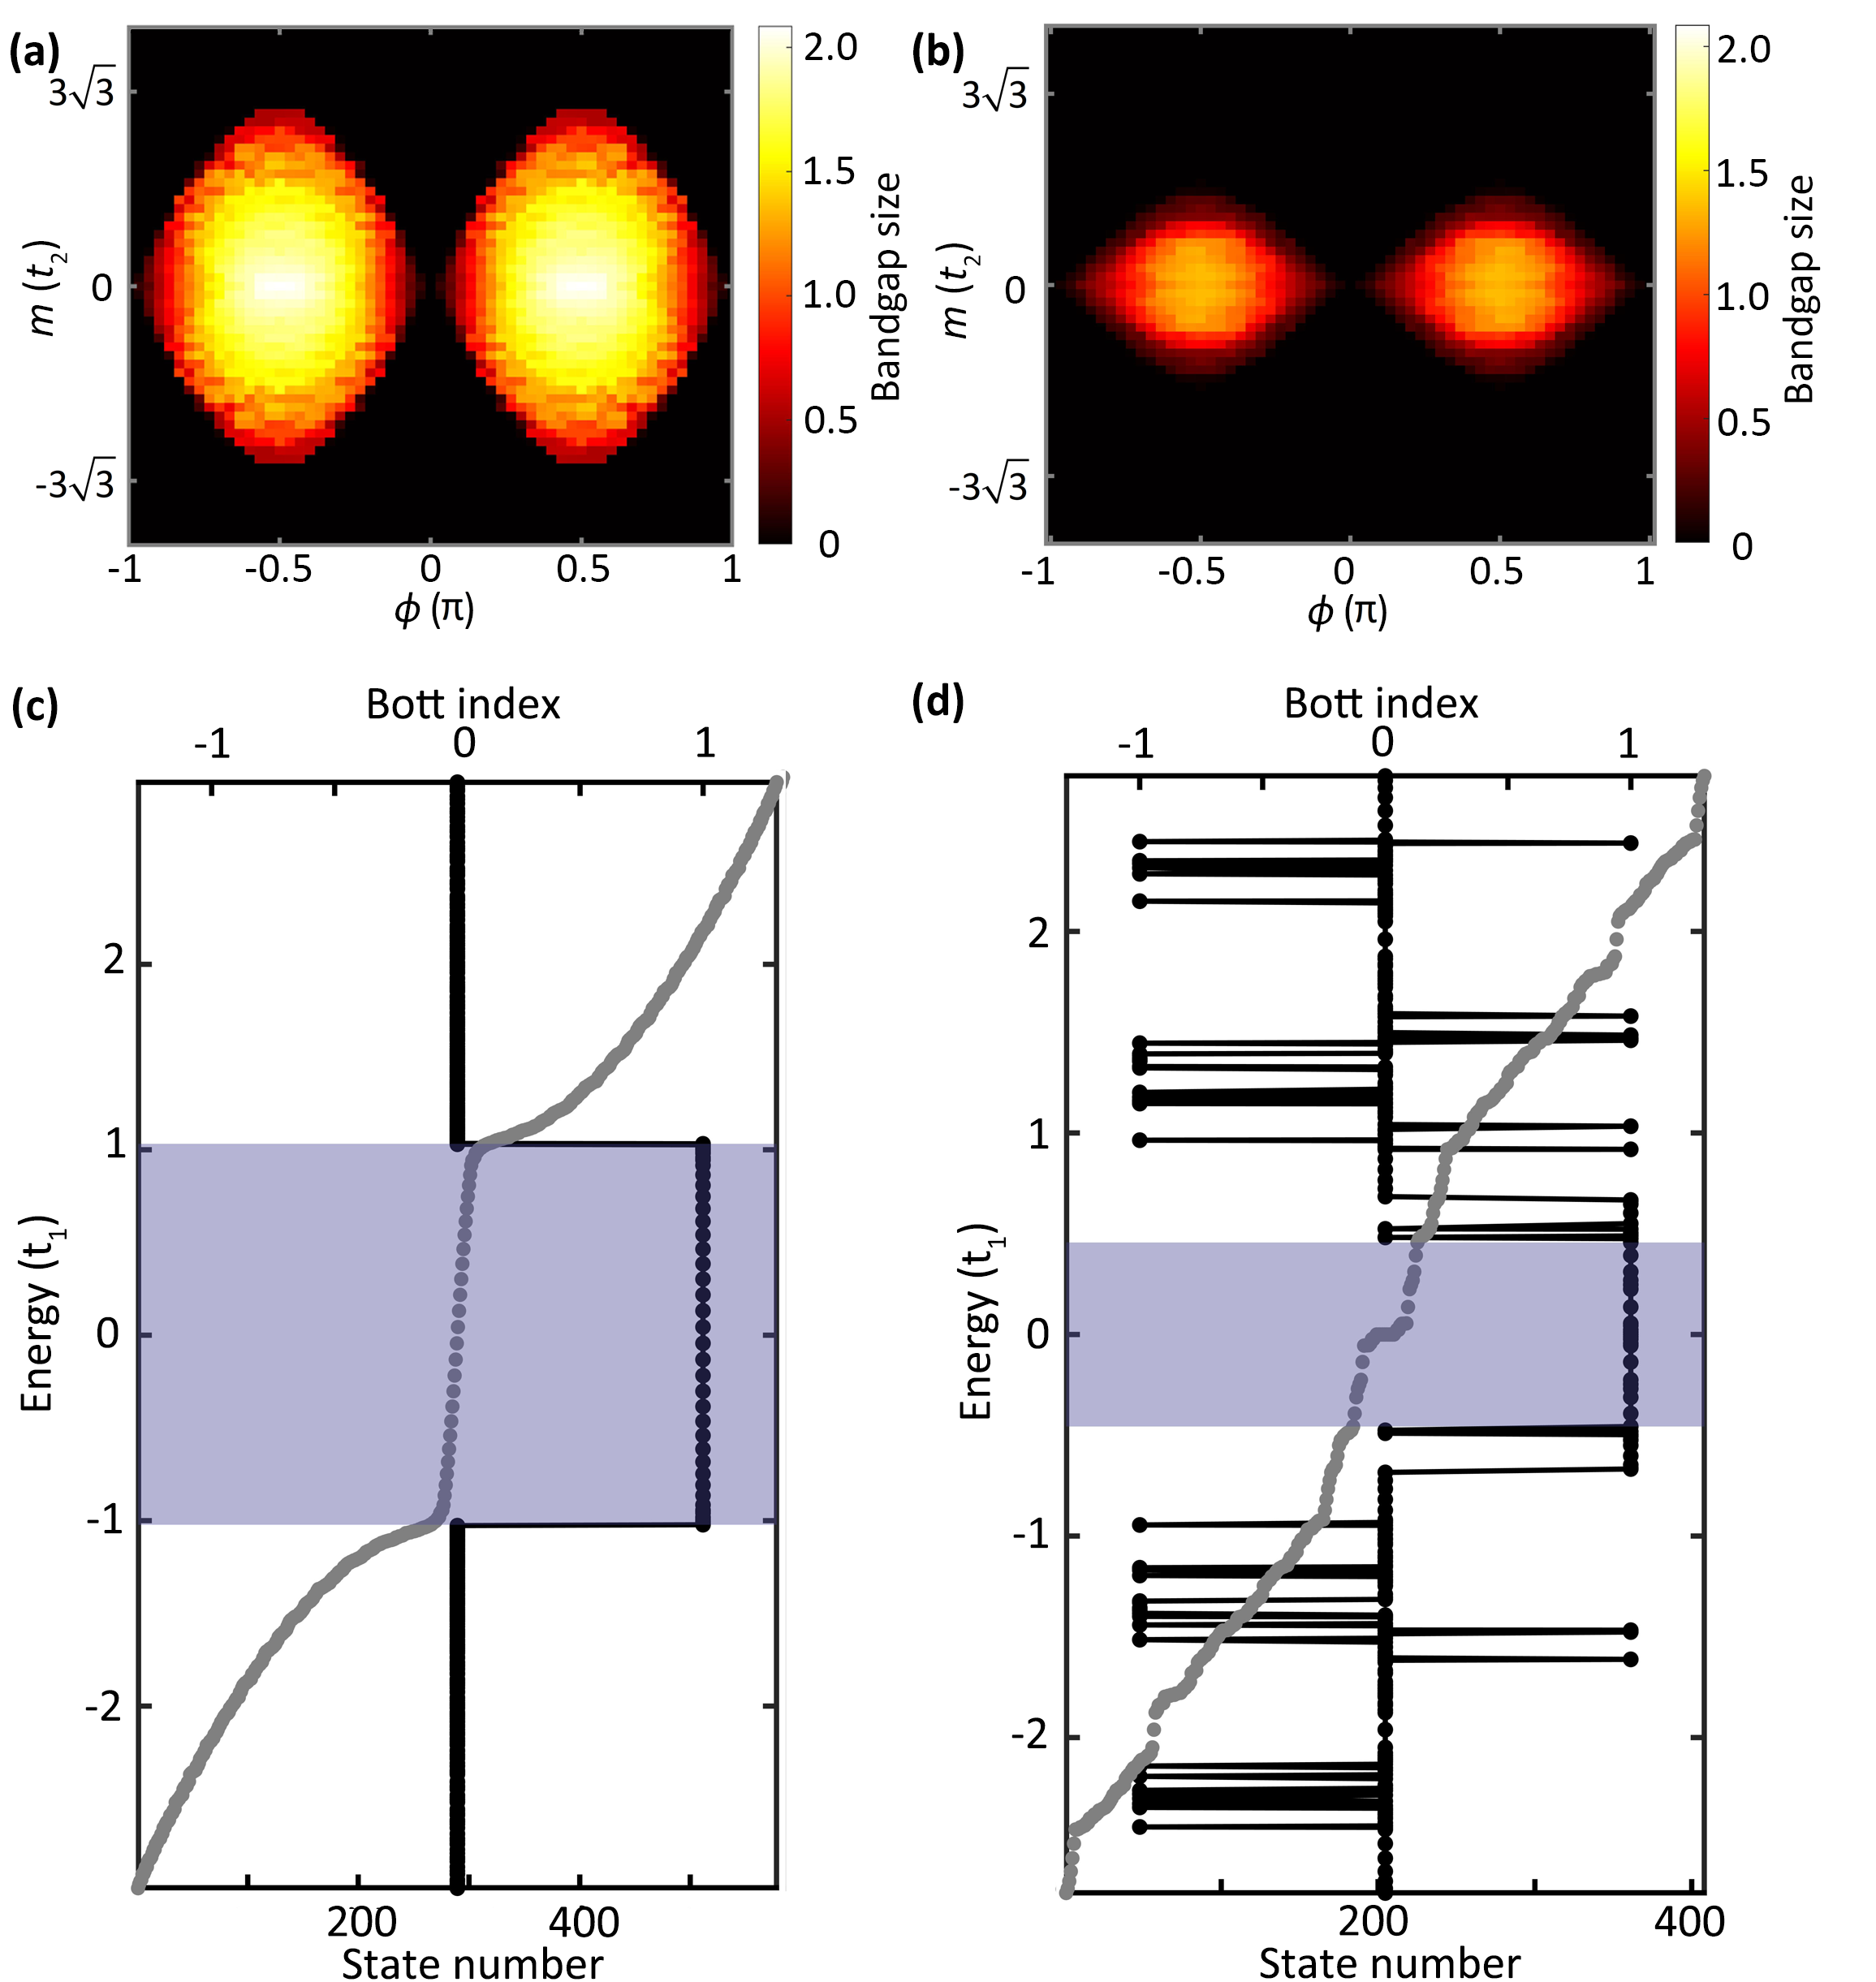
\includegraphics[width=0.5\linewidth]{FracHaldTheo/BandGap.png}
    \caption{蜂窝晶格和分形晶格的拓扑带隙}(a) 蜂窝晶格的拓扑带隙图。带隙大小通过将所有具有Bott指数为1的状态n与状态n+1之间的小带隙相加计算得出。(b) 分形晶格的拓扑带隙图。(c, d) 蜂窝晶格(c)和分形晶格(d)在最大带隙处的能谱和Bott指数结果。蓝色阴影区域对应于Bott指数为1的状态。注意,阴影区域外具有Bott指数为1的状态没有拓扑保护。
    \label{fig:BandGap}
\end{figure}

可以看到,对于蜂窝晶格,最大带隙出现在$\phi=±π/2, m=0$ 处,大小为 $\Delta E=2.085$,这与理论值 $\Delta E=6\sqrt{3}t_2=2.078$ 一致。带隙大小在拓扑相变点(灰色线,如图 1 所示)处减小至零。而在分形模型中,拓扑带隙的大小相对较小,最大带隙为 $\Delta E=1.358$,约为蜂窝晶格带隙的 $65\%$,这表明拓扑保护的强度相对较弱。需要注意的是,由于存在一些不受拓扑保护的可疑拓扑边缘态,实际带隙的大小略小于理论值。

\section{拓扑鲁棒性}

拓扑保护的能力受限于拓扑带隙的大小。为了验证分形晶格中拓扑态的鲁棒性,我们选择最大带隙($\phi = \pi/2$ 和 $m = 0$)进行研究,并通过在所有晶格位置引入随机在位势(以标准差衡量)来引入无序。

在图\ref{fig:Robust}中,我们绘制了根据由Bott系数标记的带隙大小随无序强度的变化关系。每个点对应于晶格中不同的无序实现(总共 50 个)。红色和蓝色曲线分别是蜂窝晶格和分形晶格拓扑带隙大小的平均值。可以看出,当无序强度分别达到约 2.1(蜂窝晶格)和 1.2(分形晶格)时,带隙大小减小到零,这与蜂窝晶格和分形晶格的最大拓扑带隙大小吻合良好。带隙闭合行为表明,当无序强度与拓扑带隙大小相当时,拓扑保护将失效。

\begin{figure}[htbp]
    \centering
    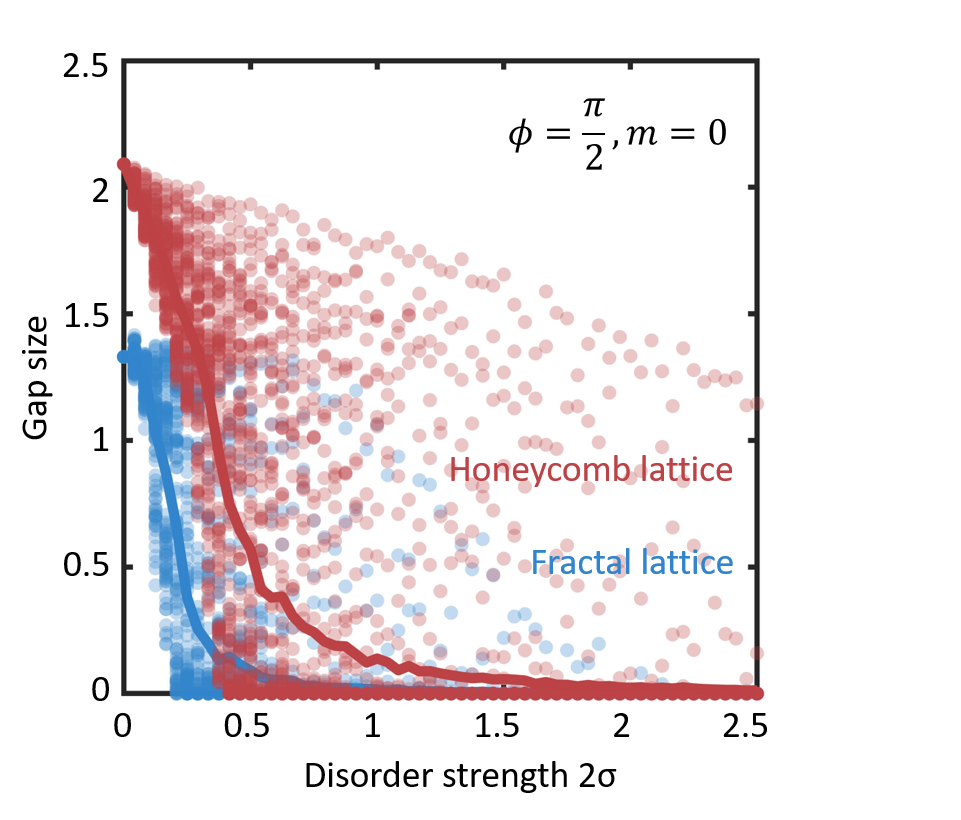
\includegraphics[width=0.5\linewidth]{FracHaldTheo/Robust.png}
    \caption{对无序的拓扑鲁棒性}蜂窝晶格和分形晶格的拓扑带隙大小(50 次实现的平均值)随无序强度的变化关系。红色和蓝色曲线分别是带隙大小的平均值。当无序强度与拓扑带隙大小相当时,拓扑保护将失效。
    \label{fig:Robust}
\end{figure}

在本节中,笔者将展示分形系统与随机缺失格点的蜂窝晶格有本质区别。如图\ref{fig:Robust}所示,通过随机删除 170 个格点(不包括最外层的格点)展示了三种蜂窝晶格的实现。此时,格点数量与分形模型相同。从图 (d-f) 的结果可以看出,具有 Bott 指数为 1 的状态非常少。我们进一步绘制了这些本征态的场分布,发现这些状态并非拓扑边缘态。

\begin{figure}[htbp]
    \centering
    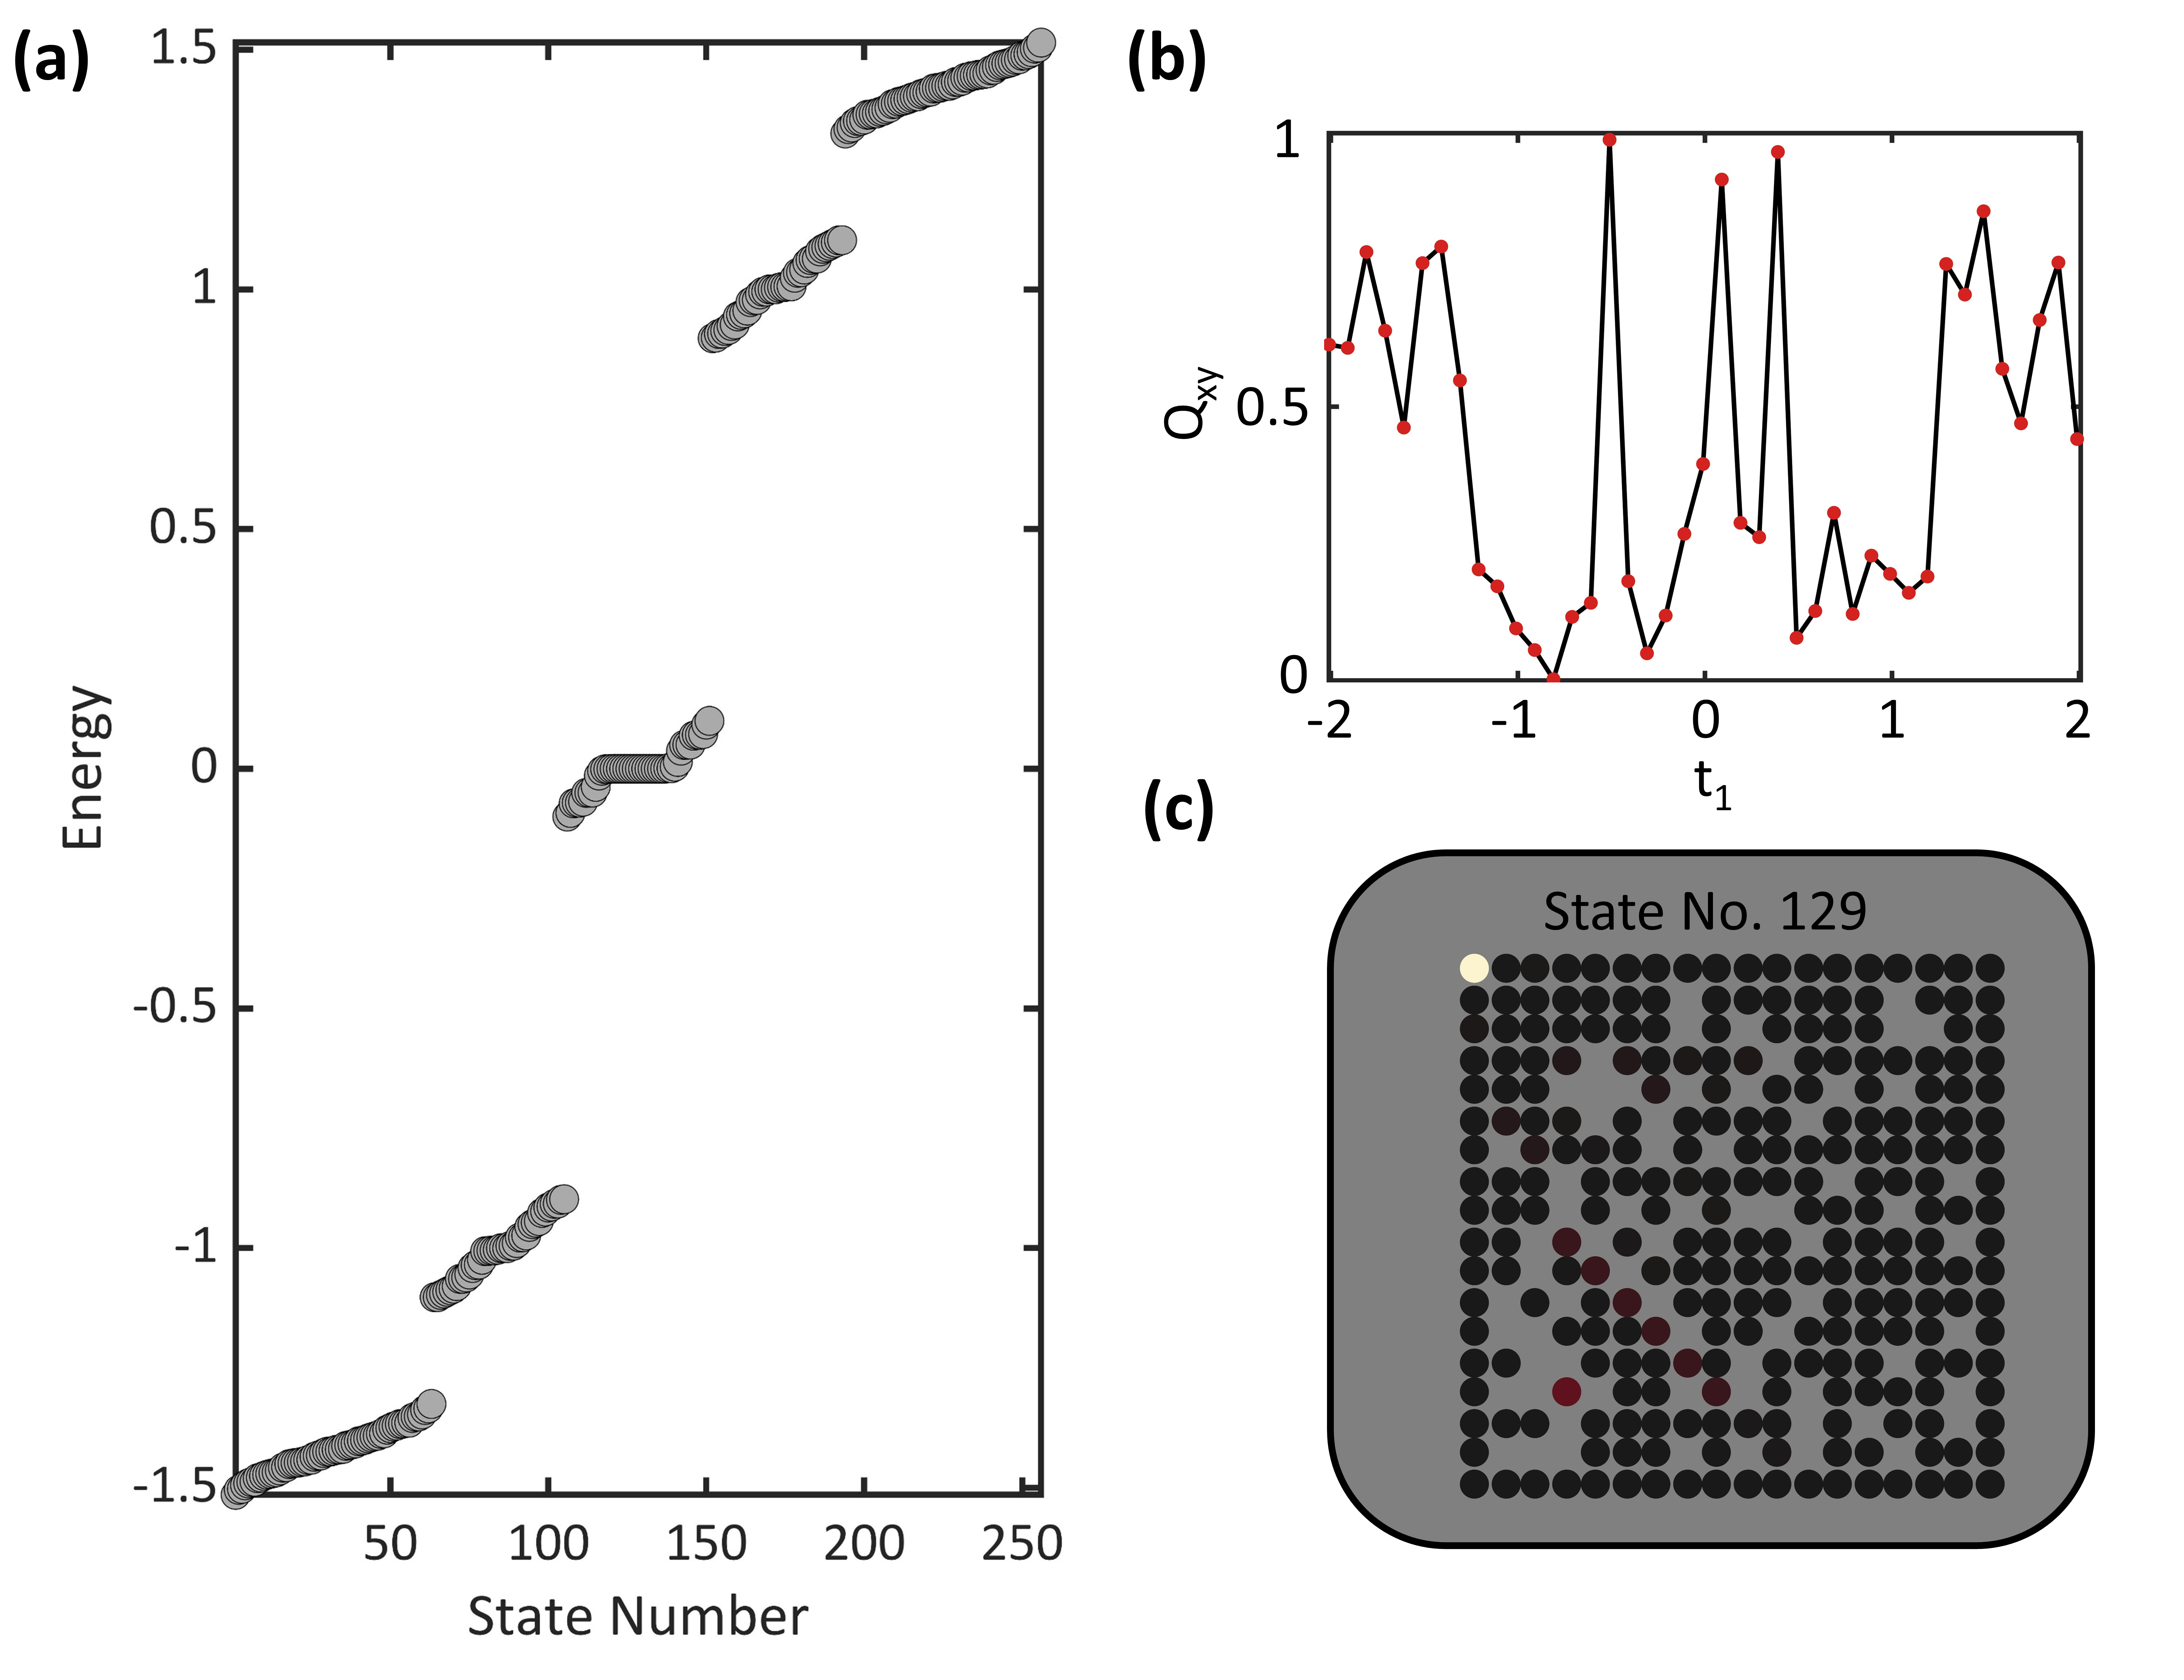
\includegraphics[width=0.75\linewidth]{FracHaldTheo/RandDel.png}
    \caption{随机删除格点}(a-c) 通过随机删除 170 个格点生成的三种蜂窝晶格实现。格点总数与分形模型相同。(d-f) 对应于 (a-c) 中晶格的 Bott 指数图。每种实现中仅有一个状态的 Bott 指数为 1。这些状态的场分布绘制在 (a-c) 中。计算参数为 $t_1 = 1$、$t_2 = 0.2$、$\phi = \pi/2$ 和 $m = 0$。
    \label{fig:RandDel}
\end{figure}

综上所述,分形系统与随机缺失格点的蜂窝晶格有本质区别,随机缺失格点的晶格不具有拓扑效应。

\section{本章小结}
本章以一个双谢宾斯基三角晶格为例,在该晶格上实现了霍尔丹模型。笔者首先介绍了该晶格的迭代产生方法,并计算其分数维度。随后笔者在该晶格上利用紧束缚模型构建了分形霍尔丹模型的哈密顿量。在该模型下,哈密顿量具有自相似能谱以及由迁移率隙而非直接带隙提供的拓扑保护,使得该分形模型与传统拓扑绝缘体截然不同。在迁移率隙中,分形晶格的内边缘态形成了许多简并的阶梯,这些简并的阶梯构成了能谱Cantor函数以及一系列特殊的混合边缘态。由于分形晶格缺乏平移对称性,本章使用Bott系数和实空间陈数作来表征分形晶格的拓扑性质。通过求解被填充本征态的Bott系数,我们计算了分形霍尔丹模型的拓扑相图,其相图被显著压缩。这种压缩现象对晶格迭代次数(晶格尺度)稳定,并且可以通过实空间陈数以及拓扑迁移率隙的关闭交叉验证。最后本章讨论了分形晶格对无序的鲁棒性以及随机删除格点于分形晶格的差异。